% =============================================================================
% 08-io-techniques-notes.tex — Lecture Notes for Week 8: I/O Techniques
% (Synchronous vs. Asynchronous I/O; Polling, Interrupts, DMA, IOP)
%
% DERIVED ARTIFACT. Source of truth: Slides/CS401/08-io-techniques.tex.
% Generated by /lecture-notes; do not hand-edit content independently of the
% Beamer source without re-running /qa-notes afterward (single-source-of-truth.md).
% Structured as a textbook chapter (numbered sections/figures/examples,
% topic-organized rather than a frame-by-frame transcript) per the project's
% textbook-chapter convention for Notes.
%
% Anchor reading: Hamacher (6th ed.) Ch. 3 (programmer's-view I/O: memory-mapped
%                 I/O, polling, interrupts, printed p.95-119) + Ch. 7 SS7.1-7.4
%                 (bus structure, synchronous/asynchronous bus operation,
%                 arbitration, interface circuits, printed p.227-242).
%                 Page-cited from master_supporting_docs/CS401/supporting_books/
%                 Hamacher2002/index.md (built 2026-08-11, 6th-edition file,
%                 page-verified via direct visual Read). DMA and IOP are NOT
%                 named in this edition (verified in the same index pass) --
%                 SS7.3 Arbitration is the functional analogue of DMA but the
%                 term is never used, so DMA/IOP content is phrased as
%                 general/standard treatment citing Stallings Ch. 8 (11th-ed.
%                 I/O chapter, confirmed in knowledge-base-CS401.md; chapter-
%                 level only, no page index yet), per
%                 .claude/rules/textbook-grounding.md. Mano Ch. 11 (chapter-level)
%                 supplies the isolated-I/O contrast; P&H (ARM ed.) Ch. 4
%                 supplies the exceptions-as-interrupts framing.
%
% Compile with: cd Notes/CS401 &&
%   TEXINPUTS=../../Preambles:$TEXINPUTS xelatex -interaction=nonstopmode 08-io-techniques-notes.tex
%   BIBINPUTS=../..:$BIBINPUTS bibtex 08-io-techniques-notes
%   TEXINPUTS=../../Preambles:$TEXINPUTS xelatex -interaction=nonstopmode 08-io-techniques-notes.tex  (x2)
%   (Windows/MiKTeX: use ; not : as the TEXINPUTS/BIBINPUTS separator)
% =============================================================================

\documentclass[11pt]{article}
\usepackage[margin=1in]{geometry}
% =============================================================================
% Preambles/header.tex — shared LaTeX/Beamer preamble for this project
%
% Use from a Beamer lecture by prepending:
%     % =============================================================================
% Preambles/header.tex — shared LaTeX/Beamer preamble for this project
%
% Use from a Beamer lecture by prepending:
%     % =============================================================================
% Preambles/header.tex — shared LaTeX/Beamer preamble for this project
%
% Use from a Beamer lecture by prepending:
%     \input{header}
% and compiling with TEXINPUTS=../Preambles:$TEXINPUTS (the /compile-latex
% skill does this automatically).
%
% PALETTE CONTRACT. Color names defined here MUST match the names in
% Quarto/theme-template.scss so Beamer and Quarto renderings use the same
% palette. The scripts/check-palette-sync.sh script enforces this.
%
% To customize: edit the HEX values below AND the matching $variable in
% Quarto/theme-template.scss, then run scripts/check-palette-sync.sh.
%
% TITLE PAGE. A formal, serif (Libertine) title-page template is defined in
% the Beamer-only block below (\setbeamertemplate{title page}) -- title,
% subtitle, a thin gold rule, then \author/\institute/\date. Frametitle and
% body text remain on Beamer's sans-serif default. No SCSS counterpart is
% needed for this (font/layout only, no new colors).
% =============================================================================

% -----------------------------------------------------------------------------
% Engine detection + encoding
%
% Our /compile-latex skill uses XeLaTeX, where inputenc is unnecessary and
% can produce encoding warnings. Only load inputenc under pdfTeX.
% -----------------------------------------------------------------------------
\usepackage{iftex}
\ifPDFTeX
  \usepackage[utf8]{inputenc}
\fi

\usepackage{amsmath, amssymb, amsthm}
\usepackage{booktabs}
\usepackage{graphicx}

% -----------------------------------------------------------------------------
% Serif face for the title page (formal/academic look). Linux Libertine is
% XeLaTeX- and pdfTeX-safe and redefines \rmdefault, so \rmfamily picks it up
% everywhere \rmfamily is used explicitly. Body text and frametitles stay on
% Beamer's own sans-serif default (unaffected) -- only the title-page
% \setbeamerfont{...} overrides below opt in to \rmfamily.
% -----------------------------------------------------------------------------
\usepackage{libertine}

% -----------------------------------------------------------------------------
% PALETTE — mirrors Quarto/theme-template.scss variable names.
% Load xcolor and define colors BEFORE anything that references them
% (notably hyperref, hypersetup, and the Beamer color assignments).
% -----------------------------------------------------------------------------
\usepackage{xcolor}

\definecolor{primary-blue}{HTML}{012169}      % headings, accents
\definecolor{primary-gold}{HTML}{B9975B}      % emphasis, borders
\definecolor{highlight-yellow}{HTML}{F2A900}  % markers, alerts
\definecolor{light-bg}{HTML}{E8EDF5}          % title / section backgrounds
\definecolor{jet}{HTML}{1A1A1A}               % body text

% Semantic colors (used in diagrams and annotations)
\definecolor{positive}{HTML}{15803D}          % good / observed / identified
\definecolor{negative}{HTML}{B91C1C}          % bad / problematic / bias
\definecolor{neutral}{HTML}{525252}           % reference / context

% Highlight accents (match .hi-* classes in the SCSS)
\definecolor{hi-slate}{HTML}{314F4F}
\definecolor{hi-green}{HTML}{2E8B57}
\definecolor{hi-red}{HTML}{C41E3A}

% Semantic aliases so skill templates and snippets can write
% \textcolor{accent}{...} without hard-coding "primary-blue".
\colorlet{accent}{primary-blue}
\colorlet{accent2}{primary-gold}

% -----------------------------------------------------------------------------
% Hyperref — loaded AFTER xcolor + palette so link colors resolve.
% -----------------------------------------------------------------------------
\usepackage{hyperref}
\hypersetup{colorlinks=true, linkcolor=primary-blue, urlcolor=primary-blue,
            citecolor=primary-blue, pdfborder={0 0 0}}

% -----------------------------------------------------------------------------
% Course code — set once per deck (after \input{header}, before \begin{document})
% via \coursecode{CS401}. Shown in the footer on every slide so a deck's course
% is identifiable without opening the title page. Empty by default.
% -----------------------------------------------------------------------------
\makeatletter
\newcommand{\coursecode}[1]{\gdef\@coursecodetext{#1}}
\gdef\@coursecodetext{}
\makeatother

% -----------------------------------------------------------------------------
% Beamer theme assignments (only apply under Beamer).
%
% We detect Beamer via \@ifclassloaded{beamer}, which is the documented,
% non-internal way. This must be wrapped in \makeatletter/\makeatother
% because \@ifclassloaded contains an @-catcode character.
% -----------------------------------------------------------------------------
\makeatletter
\@ifclassloaded{beamer}{%
  \usefonttheme{professionalfonts}
  \setbeamercolor{structure}{fg=primary-blue}
  \setbeamercolor{frametitle}{fg=primary-blue}
  \setbeamercolor{title}{fg=primary-blue}
  \setbeamercolor{subtitle}{fg=primary-gold}
  \setbeamercolor{author}{fg=primary-blue}
  \setbeamercolor{institute}{fg=neutral}
  \setbeamercolor{date}{fg=primary-gold}
  \setbeamercolor{itemize item}{fg=primary-blue}
  \setbeamercolor{itemize subitem}{fg=primary-gold}
  \setbeamercolor{alerted text}{fg=primary-gold}
  \setbeamercolor{block title}{fg=white, bg=primary-blue}
  \setbeamercolor{block body}{bg=light-bg}
  % Semantic block variants: block=definition/concept (blue), exampleblock=
  % worked example (green/positive), alertblock=key takeaway or caution (gold).
  % Keep to <=2 colored boxes per slide across ALL three variants (INV-7).
  \setbeamercolor{block title example}{fg=white, bg=positive}
  \setbeamercolor{block body example}{bg=light-bg}
  \setbeamercolor{block title alerted}{fg=white, bg=primary-gold}
  \setbeamercolor{block body alerted}{bg=light-bg}

  % ---------------------------------------------------------------------------
  % Formal title page: serif (Libertine, via \rmfamily) for title-page
  % elements only. Body text, itemize, and frametitle are intentionally left
  % on Beamer's sans-serif default -- \usebeamerfont{title} is also what
  % \transitionslide (below) uses for its big centered text, so section
  % transitions pick up the same serif treatment for free.
  % ---------------------------------------------------------------------------
  \setbeamerfont{title}{family=\rmfamily, series=\bfseries, size=\Large}
  \setbeamerfont{subtitle}{family=\rmfamily, shape=\itshape, size=\normalsize}
  \setbeamerfont{author}{family=\rmfamily, size=\normalsize}
  \setbeamerfont{institute}{family=\rmfamily, size=\scriptsize}
  \setbeamerfont{date}{family=\rmfamily, size=\scriptsize}

  \setbeamertemplate{title page}{
    \vfill
    \begin{center}
      {\usebeamerfont{title}\usebeamercolor[fg]{title}\inserttitle\par}
      \vspace{0.15cm}
      {\usebeamerfont{subtitle}\usebeamercolor[fg]{subtitle}\insertsubtitle\par}
      \vspace{0.45cm}
      {\color{primary-gold}\rule{0.42\textwidth}{0.6pt}\par}
      \vspace{0.45cm}
      {\usebeamerfont{author}\usebeamercolor[fg]{author}\insertauthor\par}
      \vspace{0.35cm}
      {\usebeamerfont{institute}\usebeamercolor[fg]{institute}\insertinstitute\par}
      \vspace{0.35cm}
      {\usebeamerfont{date}\usebeamercolor[fg]{date}\insertdate\par}
    \end{center}
    \vfill
  }

  % Minimal footer: course code (left) + page X / N (right), no navigation clutter
  \setbeamertemplate{navigation symbols}{}
  \setbeamertemplate{footline}{%
    \color{neutral}\footnotesize\hspace{0.7em}\@coursecodetext\hfill
    \insertframenumber/\inserttotalframenumber\hspace{0.7em}\vspace{0.3em}}
}{}
\makeatother

% -----------------------------------------------------------------------------
% TikZ setup — libraries the snippet gallery uses
% -----------------------------------------------------------------------------
\usepackage{tikz}
\usetikzlibrary{arrows.meta, positioning, calc, decorations.pathreplacing,
                fit, shapes.geometric, backgrounds}

% Shared TikZ styles — snippets and hand-written diagrams can pick these up
% via `\begin{tikzpicture}[every node/.style={...}]` or by naming specific
% styles (e.g., `\node[dag-node] (X) at (0,0) {X};`).
\tikzset{
  % Node styles for causal DAGs and similar
  dag-node/.style = {
    draw=primary-blue, fill=light-bg, rounded corners=2pt,
    minimum width=1.2cm, minimum height=0.9cm, align=center, font=\small
  },
  decision-node/.style = {
    draw=primary-gold, fill=white, diamond, aspect=1.8,
    minimum width=1.8cm, minimum height=1.2cm, align=center, font=\small,
    inner sep=1pt
  },
  % Edge styles — observed vs counterfactual
  observed-edge/.style = {-{Latex[length=2.5mm]}, thick, draw=jet},
  counterfactual-edge/.style = {-{Latex[length=2.5mm]}, thick, draw=neutral, dashed},
  confound-edge/.style = {-{Latex[length=2.5mm]}, thick, draw=negative, dashed},
  % Data-point styles for plots
  observed-dot/.style = {fill=primary-blue, draw=primary-blue, circle, inner sep=1.2pt},
  counterfactual-dot/.style = {fill=white, draw=neutral, circle, inner sep=1.2pt}
}

% -----------------------------------------------------------------------------
% Convenience macros
% -----------------------------------------------------------------------------
\newcommand{\muted}[1]{\textcolor{neutral}{#1}}
\newcommand{\key}[1]{\textcolor{primary-gold}{\textbf{#1}}}
\newcommand{\good}[1]{\textcolor{positive}{#1}}
\newcommand{\bad}[1]{\textcolor{negative}{#1}}

% Standout frame macro: full-bleed dark background for section transitions.
% Beamer-only (uses \begin{frame}/\setbeamercolor/\usebeamerfont) -- do not
% call from an article-class file (e.g. Notes/<CODE>/*-notes.tex). \muted,
% \key, \good, \bad, and \coursecode above are plain xcolor/gdef and are
% safe to use from either class; verified when Notes/article-class support
% was added.
% Expand: \transitionslide{Your transition title}
\newcommand{\transitionslide}[1]{%
  \begingroup
  \setbeamercolor{background canvas}{bg=primary-blue}
  \begin{frame}[plain]
    \centering
    \vfill
    {\usebeamerfont{title}\color{white}\Large #1\par}
    \vfill
  \end{frame}
  \endgroup
}

% and compiling with TEXINPUTS=../Preambles:$TEXINPUTS (the /compile-latex
% skill does this automatically).
%
% PALETTE CONTRACT. Color names defined here MUST match the names in
% Quarto/theme-template.scss so Beamer and Quarto renderings use the same
% palette. The scripts/check-palette-sync.sh script enforces this.
%
% To customize: edit the HEX values below AND the matching $variable in
% Quarto/theme-template.scss, then run scripts/check-palette-sync.sh.
%
% TITLE PAGE. A formal, serif (Libertine) title-page template is defined in
% the Beamer-only block below (\setbeamertemplate{title page}) -- title,
% subtitle, a thin gold rule, then \author/\institute/\date. Frametitle and
% body text remain on Beamer's sans-serif default. No SCSS counterpart is
% needed for this (font/layout only, no new colors).
% =============================================================================

% -----------------------------------------------------------------------------
% Engine detection + encoding
%
% Our /compile-latex skill uses XeLaTeX, where inputenc is unnecessary and
% can produce encoding warnings. Only load inputenc under pdfTeX.
% -----------------------------------------------------------------------------
\usepackage{iftex}
\ifPDFTeX
  \usepackage[utf8]{inputenc}
\fi

\usepackage{amsmath, amssymb, amsthm}
\usepackage{booktabs}
\usepackage{graphicx}

% -----------------------------------------------------------------------------
% Serif face for the title page (formal/academic look). Linux Libertine is
% XeLaTeX- and pdfTeX-safe and redefines \rmdefault, so \rmfamily picks it up
% everywhere \rmfamily is used explicitly. Body text and frametitles stay on
% Beamer's own sans-serif default (unaffected) -- only the title-page
% \setbeamerfont{...} overrides below opt in to \rmfamily.
% -----------------------------------------------------------------------------
\usepackage{libertine}

% -----------------------------------------------------------------------------
% PALETTE — mirrors Quarto/theme-template.scss variable names.
% Load xcolor and define colors BEFORE anything that references them
% (notably hyperref, hypersetup, and the Beamer color assignments).
% -----------------------------------------------------------------------------
\usepackage{xcolor}

\definecolor{primary-blue}{HTML}{012169}      % headings, accents
\definecolor{primary-gold}{HTML}{B9975B}      % emphasis, borders
\definecolor{highlight-yellow}{HTML}{F2A900}  % markers, alerts
\definecolor{light-bg}{HTML}{E8EDF5}          % title / section backgrounds
\definecolor{jet}{HTML}{1A1A1A}               % body text

% Semantic colors (used in diagrams and annotations)
\definecolor{positive}{HTML}{15803D}          % good / observed / identified
\definecolor{negative}{HTML}{B91C1C}          % bad / problematic / bias
\definecolor{neutral}{HTML}{525252}           % reference / context

% Highlight accents (match .hi-* classes in the SCSS)
\definecolor{hi-slate}{HTML}{314F4F}
\definecolor{hi-green}{HTML}{2E8B57}
\definecolor{hi-red}{HTML}{C41E3A}

% Semantic aliases so skill templates and snippets can write
% \textcolor{accent}{...} without hard-coding "primary-blue".
\colorlet{accent}{primary-blue}
\colorlet{accent2}{primary-gold}

% -----------------------------------------------------------------------------
% Hyperref — loaded AFTER xcolor + palette so link colors resolve.
% -----------------------------------------------------------------------------
\usepackage{hyperref}
\hypersetup{colorlinks=true, linkcolor=primary-blue, urlcolor=primary-blue,
            citecolor=primary-blue, pdfborder={0 0 0}}

% -----------------------------------------------------------------------------
% Course code — set once per deck (after % =============================================================================
% Preambles/header.tex — shared LaTeX/Beamer preamble for this project
%
% Use from a Beamer lecture by prepending:
%     \input{header}
% and compiling with TEXINPUTS=../Preambles:$TEXINPUTS (the /compile-latex
% skill does this automatically).
%
% PALETTE CONTRACT. Color names defined here MUST match the names in
% Quarto/theme-template.scss so Beamer and Quarto renderings use the same
% palette. The scripts/check-palette-sync.sh script enforces this.
%
% To customize: edit the HEX values below AND the matching $variable in
% Quarto/theme-template.scss, then run scripts/check-palette-sync.sh.
%
% TITLE PAGE. A formal, serif (Libertine) title-page template is defined in
% the Beamer-only block below (\setbeamertemplate{title page}) -- title,
% subtitle, a thin gold rule, then \author/\institute/\date. Frametitle and
% body text remain on Beamer's sans-serif default. No SCSS counterpart is
% needed for this (font/layout only, no new colors).
% =============================================================================

% -----------------------------------------------------------------------------
% Engine detection + encoding
%
% Our /compile-latex skill uses XeLaTeX, where inputenc is unnecessary and
% can produce encoding warnings. Only load inputenc under pdfTeX.
% -----------------------------------------------------------------------------
\usepackage{iftex}
\ifPDFTeX
  \usepackage[utf8]{inputenc}
\fi

\usepackage{amsmath, amssymb, amsthm}
\usepackage{booktabs}
\usepackage{graphicx}

% -----------------------------------------------------------------------------
% Serif face for the title page (formal/academic look). Linux Libertine is
% XeLaTeX- and pdfTeX-safe and redefines \rmdefault, so \rmfamily picks it up
% everywhere \rmfamily is used explicitly. Body text and frametitles stay on
% Beamer's own sans-serif default (unaffected) -- only the title-page
% \setbeamerfont{...} overrides below opt in to \rmfamily.
% -----------------------------------------------------------------------------
\usepackage{libertine}

% -----------------------------------------------------------------------------
% PALETTE — mirrors Quarto/theme-template.scss variable names.
% Load xcolor and define colors BEFORE anything that references them
% (notably hyperref, hypersetup, and the Beamer color assignments).
% -----------------------------------------------------------------------------
\usepackage{xcolor}

\definecolor{primary-blue}{HTML}{012169}      % headings, accents
\definecolor{primary-gold}{HTML}{B9975B}      % emphasis, borders
\definecolor{highlight-yellow}{HTML}{F2A900}  % markers, alerts
\definecolor{light-bg}{HTML}{E8EDF5}          % title / section backgrounds
\definecolor{jet}{HTML}{1A1A1A}               % body text

% Semantic colors (used in diagrams and annotations)
\definecolor{positive}{HTML}{15803D}          % good / observed / identified
\definecolor{negative}{HTML}{B91C1C}          % bad / problematic / bias
\definecolor{neutral}{HTML}{525252}           % reference / context

% Highlight accents (match .hi-* classes in the SCSS)
\definecolor{hi-slate}{HTML}{314F4F}
\definecolor{hi-green}{HTML}{2E8B57}
\definecolor{hi-red}{HTML}{C41E3A}

% Semantic aliases so skill templates and snippets can write
% \textcolor{accent}{...} without hard-coding "primary-blue".
\colorlet{accent}{primary-blue}
\colorlet{accent2}{primary-gold}

% -----------------------------------------------------------------------------
% Hyperref — loaded AFTER xcolor + palette so link colors resolve.
% -----------------------------------------------------------------------------
\usepackage{hyperref}
\hypersetup{colorlinks=true, linkcolor=primary-blue, urlcolor=primary-blue,
            citecolor=primary-blue, pdfborder={0 0 0}}

% -----------------------------------------------------------------------------
% Course code — set once per deck (after \input{header}, before \begin{document})
% via \coursecode{CS401}. Shown in the footer on every slide so a deck's course
% is identifiable without opening the title page. Empty by default.
% -----------------------------------------------------------------------------
\makeatletter
\newcommand{\coursecode}[1]{\gdef\@coursecodetext{#1}}
\gdef\@coursecodetext{}
\makeatother

% -----------------------------------------------------------------------------
% Beamer theme assignments (only apply under Beamer).
%
% We detect Beamer via \@ifclassloaded{beamer}, which is the documented,
% non-internal way. This must be wrapped in \makeatletter/\makeatother
% because \@ifclassloaded contains an @-catcode character.
% -----------------------------------------------------------------------------
\makeatletter
\@ifclassloaded{beamer}{%
  \usefonttheme{professionalfonts}
  \setbeamercolor{structure}{fg=primary-blue}
  \setbeamercolor{frametitle}{fg=primary-blue}
  \setbeamercolor{title}{fg=primary-blue}
  \setbeamercolor{subtitle}{fg=primary-gold}
  \setbeamercolor{author}{fg=primary-blue}
  \setbeamercolor{institute}{fg=neutral}
  \setbeamercolor{date}{fg=primary-gold}
  \setbeamercolor{itemize item}{fg=primary-blue}
  \setbeamercolor{itemize subitem}{fg=primary-gold}
  \setbeamercolor{alerted text}{fg=primary-gold}
  \setbeamercolor{block title}{fg=white, bg=primary-blue}
  \setbeamercolor{block body}{bg=light-bg}
  % Semantic block variants: block=definition/concept (blue), exampleblock=
  % worked example (green/positive), alertblock=key takeaway or caution (gold).
  % Keep to <=2 colored boxes per slide across ALL three variants (INV-7).
  \setbeamercolor{block title example}{fg=white, bg=positive}
  \setbeamercolor{block body example}{bg=light-bg}
  \setbeamercolor{block title alerted}{fg=white, bg=primary-gold}
  \setbeamercolor{block body alerted}{bg=light-bg}

  % ---------------------------------------------------------------------------
  % Formal title page: serif (Libertine, via \rmfamily) for title-page
  % elements only. Body text, itemize, and frametitle are intentionally left
  % on Beamer's sans-serif default -- \usebeamerfont{title} is also what
  % \transitionslide (below) uses for its big centered text, so section
  % transitions pick up the same serif treatment for free.
  % ---------------------------------------------------------------------------
  \setbeamerfont{title}{family=\rmfamily, series=\bfseries, size=\Large}
  \setbeamerfont{subtitle}{family=\rmfamily, shape=\itshape, size=\normalsize}
  \setbeamerfont{author}{family=\rmfamily, size=\normalsize}
  \setbeamerfont{institute}{family=\rmfamily, size=\scriptsize}
  \setbeamerfont{date}{family=\rmfamily, size=\scriptsize}

  \setbeamertemplate{title page}{
    \vfill
    \begin{center}
      {\usebeamerfont{title}\usebeamercolor[fg]{title}\inserttitle\par}
      \vspace{0.15cm}
      {\usebeamerfont{subtitle}\usebeamercolor[fg]{subtitle}\insertsubtitle\par}
      \vspace{0.45cm}
      {\color{primary-gold}\rule{0.42\textwidth}{0.6pt}\par}
      \vspace{0.45cm}
      {\usebeamerfont{author}\usebeamercolor[fg]{author}\insertauthor\par}
      \vspace{0.35cm}
      {\usebeamerfont{institute}\usebeamercolor[fg]{institute}\insertinstitute\par}
      \vspace{0.35cm}
      {\usebeamerfont{date}\usebeamercolor[fg]{date}\insertdate\par}
    \end{center}
    \vfill
  }

  % Minimal footer: course code (left) + page X / N (right), no navigation clutter
  \setbeamertemplate{navigation symbols}{}
  \setbeamertemplate{footline}{%
    \color{neutral}\footnotesize\hspace{0.7em}\@coursecodetext\hfill
    \insertframenumber/\inserttotalframenumber\hspace{0.7em}\vspace{0.3em}}
}{}
\makeatother

% -----------------------------------------------------------------------------
% TikZ setup — libraries the snippet gallery uses
% -----------------------------------------------------------------------------
\usepackage{tikz}
\usetikzlibrary{arrows.meta, positioning, calc, decorations.pathreplacing,
                fit, shapes.geometric, backgrounds}

% Shared TikZ styles — snippets and hand-written diagrams can pick these up
% via `\begin{tikzpicture}[every node/.style={...}]` or by naming specific
% styles (e.g., `\node[dag-node] (X) at (0,0) {X};`).
\tikzset{
  % Node styles for causal DAGs and similar
  dag-node/.style = {
    draw=primary-blue, fill=light-bg, rounded corners=2pt,
    minimum width=1.2cm, minimum height=0.9cm, align=center, font=\small
  },
  decision-node/.style = {
    draw=primary-gold, fill=white, diamond, aspect=1.8,
    minimum width=1.8cm, minimum height=1.2cm, align=center, font=\small,
    inner sep=1pt
  },
  % Edge styles — observed vs counterfactual
  observed-edge/.style = {-{Latex[length=2.5mm]}, thick, draw=jet},
  counterfactual-edge/.style = {-{Latex[length=2.5mm]}, thick, draw=neutral, dashed},
  confound-edge/.style = {-{Latex[length=2.5mm]}, thick, draw=negative, dashed},
  % Data-point styles for plots
  observed-dot/.style = {fill=primary-blue, draw=primary-blue, circle, inner sep=1.2pt},
  counterfactual-dot/.style = {fill=white, draw=neutral, circle, inner sep=1.2pt}
}

% -----------------------------------------------------------------------------
% Convenience macros
% -----------------------------------------------------------------------------
\newcommand{\muted}[1]{\textcolor{neutral}{#1}}
\newcommand{\key}[1]{\textcolor{primary-gold}{\textbf{#1}}}
\newcommand{\good}[1]{\textcolor{positive}{#1}}
\newcommand{\bad}[1]{\textcolor{negative}{#1}}

% Standout frame macro: full-bleed dark background for section transitions.
% Beamer-only (uses \begin{frame}/\setbeamercolor/\usebeamerfont) -- do not
% call from an article-class file (e.g. Notes/<CODE>/*-notes.tex). \muted,
% \key, \good, \bad, and \coursecode above are plain xcolor/gdef and are
% safe to use from either class; verified when Notes/article-class support
% was added.
% Expand: \transitionslide{Your transition title}
\newcommand{\transitionslide}[1]{%
  \begingroup
  \setbeamercolor{background canvas}{bg=primary-blue}
  \begin{frame}[plain]
    \centering
    \vfill
    {\usebeamerfont{title}\color{white}\Large #1\par}
    \vfill
  \end{frame}
  \endgroup
}
, before \begin{document})
% via \coursecode{CS401}. Shown in the footer on every slide so a deck's course
% is identifiable without opening the title page. Empty by default.
% -----------------------------------------------------------------------------
\makeatletter
\newcommand{\coursecode}[1]{\gdef\@coursecodetext{#1}}
\gdef\@coursecodetext{}
\makeatother

% -----------------------------------------------------------------------------
% Beamer theme assignments (only apply under Beamer).
%
% We detect Beamer via \@ifclassloaded{beamer}, which is the documented,
% non-internal way. This must be wrapped in \makeatletter/\makeatother
% because \@ifclassloaded contains an @-catcode character.
% -----------------------------------------------------------------------------
\makeatletter
\@ifclassloaded{beamer}{%
  \usefonttheme{professionalfonts}
  \setbeamercolor{structure}{fg=primary-blue}
  \setbeamercolor{frametitle}{fg=primary-blue}
  \setbeamercolor{title}{fg=primary-blue}
  \setbeamercolor{subtitle}{fg=primary-gold}
  \setbeamercolor{author}{fg=primary-blue}
  \setbeamercolor{institute}{fg=neutral}
  \setbeamercolor{date}{fg=primary-gold}
  \setbeamercolor{itemize item}{fg=primary-blue}
  \setbeamercolor{itemize subitem}{fg=primary-gold}
  \setbeamercolor{alerted text}{fg=primary-gold}
  \setbeamercolor{block title}{fg=white, bg=primary-blue}
  \setbeamercolor{block body}{bg=light-bg}
  % Semantic block variants: block=definition/concept (blue), exampleblock=
  % worked example (green/positive), alertblock=key takeaway or caution (gold).
  % Keep to <=2 colored boxes per slide across ALL three variants (INV-7).
  \setbeamercolor{block title example}{fg=white, bg=positive}
  \setbeamercolor{block body example}{bg=light-bg}
  \setbeamercolor{block title alerted}{fg=white, bg=primary-gold}
  \setbeamercolor{block body alerted}{bg=light-bg}

  % ---------------------------------------------------------------------------
  % Formal title page: serif (Libertine, via \rmfamily) for title-page
  % elements only. Body text, itemize, and frametitle are intentionally left
  % on Beamer's sans-serif default -- \usebeamerfont{title} is also what
  % \transitionslide (below) uses for its big centered text, so section
  % transitions pick up the same serif treatment for free.
  % ---------------------------------------------------------------------------
  \setbeamerfont{title}{family=\rmfamily, series=\bfseries, size=\Large}
  \setbeamerfont{subtitle}{family=\rmfamily, shape=\itshape, size=\normalsize}
  \setbeamerfont{author}{family=\rmfamily, size=\normalsize}
  \setbeamerfont{institute}{family=\rmfamily, size=\scriptsize}
  \setbeamerfont{date}{family=\rmfamily, size=\scriptsize}

  \setbeamertemplate{title page}{
    \vfill
    \begin{center}
      {\usebeamerfont{title}\usebeamercolor[fg]{title}\inserttitle\par}
      \vspace{0.15cm}
      {\usebeamerfont{subtitle}\usebeamercolor[fg]{subtitle}\insertsubtitle\par}
      \vspace{0.45cm}
      {\color{primary-gold}\rule{0.42\textwidth}{0.6pt}\par}
      \vspace{0.45cm}
      {\usebeamerfont{author}\usebeamercolor[fg]{author}\insertauthor\par}
      \vspace{0.35cm}
      {\usebeamerfont{institute}\usebeamercolor[fg]{institute}\insertinstitute\par}
      \vspace{0.35cm}
      {\usebeamerfont{date}\usebeamercolor[fg]{date}\insertdate\par}
    \end{center}
    \vfill
  }

  % Minimal footer: course code (left) + page X / N (right), no navigation clutter
  \setbeamertemplate{navigation symbols}{}
  \setbeamertemplate{footline}{%
    \color{neutral}\footnotesize\hspace{0.7em}\@coursecodetext\hfill
    \insertframenumber/\inserttotalframenumber\hspace{0.7em}\vspace{0.3em}}
}{}
\makeatother

% -----------------------------------------------------------------------------
% TikZ setup — libraries the snippet gallery uses
% -----------------------------------------------------------------------------
\usepackage{tikz}
\usetikzlibrary{arrows.meta, positioning, calc, decorations.pathreplacing,
                fit, shapes.geometric, backgrounds}

% Shared TikZ styles — snippets and hand-written diagrams can pick these up
% via `\begin{tikzpicture}[every node/.style={...}]` or by naming specific
% styles (e.g., `\node[dag-node] (X) at (0,0) {X};`).
\tikzset{
  % Node styles for causal DAGs and similar
  dag-node/.style = {
    draw=primary-blue, fill=light-bg, rounded corners=2pt,
    minimum width=1.2cm, minimum height=0.9cm, align=center, font=\small
  },
  decision-node/.style = {
    draw=primary-gold, fill=white, diamond, aspect=1.8,
    minimum width=1.8cm, minimum height=1.2cm, align=center, font=\small,
    inner sep=1pt
  },
  % Edge styles — observed vs counterfactual
  observed-edge/.style = {-{Latex[length=2.5mm]}, thick, draw=jet},
  counterfactual-edge/.style = {-{Latex[length=2.5mm]}, thick, draw=neutral, dashed},
  confound-edge/.style = {-{Latex[length=2.5mm]}, thick, draw=negative, dashed},
  % Data-point styles for plots
  observed-dot/.style = {fill=primary-blue, draw=primary-blue, circle, inner sep=1.2pt},
  counterfactual-dot/.style = {fill=white, draw=neutral, circle, inner sep=1.2pt}
}

% -----------------------------------------------------------------------------
% Convenience macros
% -----------------------------------------------------------------------------
\newcommand{\muted}[1]{\textcolor{neutral}{#1}}
\newcommand{\key}[1]{\textcolor{primary-gold}{\textbf{#1}}}
\newcommand{\good}[1]{\textcolor{positive}{#1}}
\newcommand{\bad}[1]{\textcolor{negative}{#1}}

% Standout frame macro: full-bleed dark background for section transitions.
% Beamer-only (uses \begin{frame}/\setbeamercolor/\usebeamerfont) -- do not
% call from an article-class file (e.g. Notes/<CODE>/*-notes.tex). \muted,
% \key, \good, \bad, and \coursecode above are plain xcolor/gdef and are
% safe to use from either class; verified when Notes/article-class support
% was added.
% Expand: \transitionslide{Your transition title}
\newcommand{\transitionslide}[1]{%
  \begingroup
  \setbeamercolor{background canvas}{bg=primary-blue}
  \begin{frame}[plain]
    \centering
    \vfill
    {\usebeamerfont{title}\color{white}\Large #1\par}
    \vfill
  \end{frame}
  \endgroup
}

% and compiling with TEXINPUTS=../Preambles:$TEXINPUTS (the /compile-latex
% skill does this automatically).
%
% PALETTE CONTRACT. Color names defined here MUST match the names in
% Quarto/theme-template.scss so Beamer and Quarto renderings use the same
% palette. The scripts/check-palette-sync.sh script enforces this.
%
% To customize: edit the HEX values below AND the matching $variable in
% Quarto/theme-template.scss, then run scripts/check-palette-sync.sh.
%
% TITLE PAGE. A formal, serif (Libertine) title-page template is defined in
% the Beamer-only block below (\setbeamertemplate{title page}) -- title,
% subtitle, a thin gold rule, then \author/\institute/\date. Frametitle and
% body text remain on Beamer's sans-serif default. No SCSS counterpart is
% needed for this (font/layout only, no new colors).
% =============================================================================

% -----------------------------------------------------------------------------
% Engine detection + encoding
%
% Our /compile-latex skill uses XeLaTeX, where inputenc is unnecessary and
% can produce encoding warnings. Only load inputenc under pdfTeX.
% -----------------------------------------------------------------------------
\usepackage{iftex}
\ifPDFTeX
  \usepackage[utf8]{inputenc}
\fi

\usepackage{amsmath, amssymb, amsthm}
\usepackage{booktabs}
\usepackage{graphicx}

% -----------------------------------------------------------------------------
% Serif face for the title page (formal/academic look). Linux Libertine is
% XeLaTeX- and pdfTeX-safe and redefines \rmdefault, so \rmfamily picks it up
% everywhere \rmfamily is used explicitly. Body text and frametitles stay on
% Beamer's own sans-serif default (unaffected) -- only the title-page
% \setbeamerfont{...} overrides below opt in to \rmfamily.
% -----------------------------------------------------------------------------
\usepackage{libertine}

% -----------------------------------------------------------------------------
% PALETTE — mirrors Quarto/theme-template.scss variable names.
% Load xcolor and define colors BEFORE anything that references them
% (notably hyperref, hypersetup, and the Beamer color assignments).
% -----------------------------------------------------------------------------
\usepackage{xcolor}

\definecolor{primary-blue}{HTML}{012169}      % headings, accents
\definecolor{primary-gold}{HTML}{B9975B}      % emphasis, borders
\definecolor{highlight-yellow}{HTML}{F2A900}  % markers, alerts
\definecolor{light-bg}{HTML}{E8EDF5}          % title / section backgrounds
\definecolor{jet}{HTML}{1A1A1A}               % body text

% Semantic colors (used in diagrams and annotations)
\definecolor{positive}{HTML}{15803D}          % good / observed / identified
\definecolor{negative}{HTML}{B91C1C}          % bad / problematic / bias
\definecolor{neutral}{HTML}{525252}           % reference / context

% Highlight accents (match .hi-* classes in the SCSS)
\definecolor{hi-slate}{HTML}{314F4F}
\definecolor{hi-green}{HTML}{2E8B57}
\definecolor{hi-red}{HTML}{C41E3A}

% Semantic aliases so skill templates and snippets can write
% \textcolor{accent}{...} without hard-coding "primary-blue".
\colorlet{accent}{primary-blue}
\colorlet{accent2}{primary-gold}

% -----------------------------------------------------------------------------
% Hyperref — loaded AFTER xcolor + palette so link colors resolve.
% -----------------------------------------------------------------------------
\usepackage{hyperref}
\hypersetup{colorlinks=true, linkcolor=primary-blue, urlcolor=primary-blue,
            citecolor=primary-blue, pdfborder={0 0 0}}

% -----------------------------------------------------------------------------
% Course code — set once per deck (after % =============================================================================
% Preambles/header.tex — shared LaTeX/Beamer preamble for this project
%
% Use from a Beamer lecture by prepending:
%     % =============================================================================
% Preambles/header.tex — shared LaTeX/Beamer preamble for this project
%
% Use from a Beamer lecture by prepending:
%     \input{header}
% and compiling with TEXINPUTS=../Preambles:$TEXINPUTS (the /compile-latex
% skill does this automatically).
%
% PALETTE CONTRACT. Color names defined here MUST match the names in
% Quarto/theme-template.scss so Beamer and Quarto renderings use the same
% palette. The scripts/check-palette-sync.sh script enforces this.
%
% To customize: edit the HEX values below AND the matching $variable in
% Quarto/theme-template.scss, then run scripts/check-palette-sync.sh.
%
% TITLE PAGE. A formal, serif (Libertine) title-page template is defined in
% the Beamer-only block below (\setbeamertemplate{title page}) -- title,
% subtitle, a thin gold rule, then \author/\institute/\date. Frametitle and
% body text remain on Beamer's sans-serif default. No SCSS counterpart is
% needed for this (font/layout only, no new colors).
% =============================================================================

% -----------------------------------------------------------------------------
% Engine detection + encoding
%
% Our /compile-latex skill uses XeLaTeX, where inputenc is unnecessary and
% can produce encoding warnings. Only load inputenc under pdfTeX.
% -----------------------------------------------------------------------------
\usepackage{iftex}
\ifPDFTeX
  \usepackage[utf8]{inputenc}
\fi

\usepackage{amsmath, amssymb, amsthm}
\usepackage{booktabs}
\usepackage{graphicx}

% -----------------------------------------------------------------------------
% Serif face for the title page (formal/academic look). Linux Libertine is
% XeLaTeX- and pdfTeX-safe and redefines \rmdefault, so \rmfamily picks it up
% everywhere \rmfamily is used explicitly. Body text and frametitles stay on
% Beamer's own sans-serif default (unaffected) -- only the title-page
% \setbeamerfont{...} overrides below opt in to \rmfamily.
% -----------------------------------------------------------------------------
\usepackage{libertine}

% -----------------------------------------------------------------------------
% PALETTE — mirrors Quarto/theme-template.scss variable names.
% Load xcolor and define colors BEFORE anything that references them
% (notably hyperref, hypersetup, and the Beamer color assignments).
% -----------------------------------------------------------------------------
\usepackage{xcolor}

\definecolor{primary-blue}{HTML}{012169}      % headings, accents
\definecolor{primary-gold}{HTML}{B9975B}      % emphasis, borders
\definecolor{highlight-yellow}{HTML}{F2A900}  % markers, alerts
\definecolor{light-bg}{HTML}{E8EDF5}          % title / section backgrounds
\definecolor{jet}{HTML}{1A1A1A}               % body text

% Semantic colors (used in diagrams and annotations)
\definecolor{positive}{HTML}{15803D}          % good / observed / identified
\definecolor{negative}{HTML}{B91C1C}          % bad / problematic / bias
\definecolor{neutral}{HTML}{525252}           % reference / context

% Highlight accents (match .hi-* classes in the SCSS)
\definecolor{hi-slate}{HTML}{314F4F}
\definecolor{hi-green}{HTML}{2E8B57}
\definecolor{hi-red}{HTML}{C41E3A}

% Semantic aliases so skill templates and snippets can write
% \textcolor{accent}{...} without hard-coding "primary-blue".
\colorlet{accent}{primary-blue}
\colorlet{accent2}{primary-gold}

% -----------------------------------------------------------------------------
% Hyperref — loaded AFTER xcolor + palette so link colors resolve.
% -----------------------------------------------------------------------------
\usepackage{hyperref}
\hypersetup{colorlinks=true, linkcolor=primary-blue, urlcolor=primary-blue,
            citecolor=primary-blue, pdfborder={0 0 0}}

% -----------------------------------------------------------------------------
% Course code — set once per deck (after \input{header}, before \begin{document})
% via \coursecode{CS401}. Shown in the footer on every slide so a deck's course
% is identifiable without opening the title page. Empty by default.
% -----------------------------------------------------------------------------
\makeatletter
\newcommand{\coursecode}[1]{\gdef\@coursecodetext{#1}}
\gdef\@coursecodetext{}
\makeatother

% -----------------------------------------------------------------------------
% Beamer theme assignments (only apply under Beamer).
%
% We detect Beamer via \@ifclassloaded{beamer}, which is the documented,
% non-internal way. This must be wrapped in \makeatletter/\makeatother
% because \@ifclassloaded contains an @-catcode character.
% -----------------------------------------------------------------------------
\makeatletter
\@ifclassloaded{beamer}{%
  \usefonttheme{professionalfonts}
  \setbeamercolor{structure}{fg=primary-blue}
  \setbeamercolor{frametitle}{fg=primary-blue}
  \setbeamercolor{title}{fg=primary-blue}
  \setbeamercolor{subtitle}{fg=primary-gold}
  \setbeamercolor{author}{fg=primary-blue}
  \setbeamercolor{institute}{fg=neutral}
  \setbeamercolor{date}{fg=primary-gold}
  \setbeamercolor{itemize item}{fg=primary-blue}
  \setbeamercolor{itemize subitem}{fg=primary-gold}
  \setbeamercolor{alerted text}{fg=primary-gold}
  \setbeamercolor{block title}{fg=white, bg=primary-blue}
  \setbeamercolor{block body}{bg=light-bg}
  % Semantic block variants: block=definition/concept (blue), exampleblock=
  % worked example (green/positive), alertblock=key takeaway or caution (gold).
  % Keep to <=2 colored boxes per slide across ALL three variants (INV-7).
  \setbeamercolor{block title example}{fg=white, bg=positive}
  \setbeamercolor{block body example}{bg=light-bg}
  \setbeamercolor{block title alerted}{fg=white, bg=primary-gold}
  \setbeamercolor{block body alerted}{bg=light-bg}

  % ---------------------------------------------------------------------------
  % Formal title page: serif (Libertine, via \rmfamily) for title-page
  % elements only. Body text, itemize, and frametitle are intentionally left
  % on Beamer's sans-serif default -- \usebeamerfont{title} is also what
  % \transitionslide (below) uses for its big centered text, so section
  % transitions pick up the same serif treatment for free.
  % ---------------------------------------------------------------------------
  \setbeamerfont{title}{family=\rmfamily, series=\bfseries, size=\Large}
  \setbeamerfont{subtitle}{family=\rmfamily, shape=\itshape, size=\normalsize}
  \setbeamerfont{author}{family=\rmfamily, size=\normalsize}
  \setbeamerfont{institute}{family=\rmfamily, size=\scriptsize}
  \setbeamerfont{date}{family=\rmfamily, size=\scriptsize}

  \setbeamertemplate{title page}{
    \vfill
    \begin{center}
      {\usebeamerfont{title}\usebeamercolor[fg]{title}\inserttitle\par}
      \vspace{0.15cm}
      {\usebeamerfont{subtitle}\usebeamercolor[fg]{subtitle}\insertsubtitle\par}
      \vspace{0.45cm}
      {\color{primary-gold}\rule{0.42\textwidth}{0.6pt}\par}
      \vspace{0.45cm}
      {\usebeamerfont{author}\usebeamercolor[fg]{author}\insertauthor\par}
      \vspace{0.35cm}
      {\usebeamerfont{institute}\usebeamercolor[fg]{institute}\insertinstitute\par}
      \vspace{0.35cm}
      {\usebeamerfont{date}\usebeamercolor[fg]{date}\insertdate\par}
    \end{center}
    \vfill
  }

  % Minimal footer: course code (left) + page X / N (right), no navigation clutter
  \setbeamertemplate{navigation symbols}{}
  \setbeamertemplate{footline}{%
    \color{neutral}\footnotesize\hspace{0.7em}\@coursecodetext\hfill
    \insertframenumber/\inserttotalframenumber\hspace{0.7em}\vspace{0.3em}}
}{}
\makeatother

% -----------------------------------------------------------------------------
% TikZ setup — libraries the snippet gallery uses
% -----------------------------------------------------------------------------
\usepackage{tikz}
\usetikzlibrary{arrows.meta, positioning, calc, decorations.pathreplacing,
                fit, shapes.geometric, backgrounds}

% Shared TikZ styles — snippets and hand-written diagrams can pick these up
% via `\begin{tikzpicture}[every node/.style={...}]` or by naming specific
% styles (e.g., `\node[dag-node] (X) at (0,0) {X};`).
\tikzset{
  % Node styles for causal DAGs and similar
  dag-node/.style = {
    draw=primary-blue, fill=light-bg, rounded corners=2pt,
    minimum width=1.2cm, minimum height=0.9cm, align=center, font=\small
  },
  decision-node/.style = {
    draw=primary-gold, fill=white, diamond, aspect=1.8,
    minimum width=1.8cm, minimum height=1.2cm, align=center, font=\small,
    inner sep=1pt
  },
  % Edge styles — observed vs counterfactual
  observed-edge/.style = {-{Latex[length=2.5mm]}, thick, draw=jet},
  counterfactual-edge/.style = {-{Latex[length=2.5mm]}, thick, draw=neutral, dashed},
  confound-edge/.style = {-{Latex[length=2.5mm]}, thick, draw=negative, dashed},
  % Data-point styles for plots
  observed-dot/.style = {fill=primary-blue, draw=primary-blue, circle, inner sep=1.2pt},
  counterfactual-dot/.style = {fill=white, draw=neutral, circle, inner sep=1.2pt}
}

% -----------------------------------------------------------------------------
% Convenience macros
% -----------------------------------------------------------------------------
\newcommand{\muted}[1]{\textcolor{neutral}{#1}}
\newcommand{\key}[1]{\textcolor{primary-gold}{\textbf{#1}}}
\newcommand{\good}[1]{\textcolor{positive}{#1}}
\newcommand{\bad}[1]{\textcolor{negative}{#1}}

% Standout frame macro: full-bleed dark background for section transitions.
% Beamer-only (uses \begin{frame}/\setbeamercolor/\usebeamerfont) -- do not
% call from an article-class file (e.g. Notes/<CODE>/*-notes.tex). \muted,
% \key, \good, \bad, and \coursecode above are plain xcolor/gdef and are
% safe to use from either class; verified when Notes/article-class support
% was added.
% Expand: \transitionslide{Your transition title}
\newcommand{\transitionslide}[1]{%
  \begingroup
  \setbeamercolor{background canvas}{bg=primary-blue}
  \begin{frame}[plain]
    \centering
    \vfill
    {\usebeamerfont{title}\color{white}\Large #1\par}
    \vfill
  \end{frame}
  \endgroup
}

% and compiling with TEXINPUTS=../Preambles:$TEXINPUTS (the /compile-latex
% skill does this automatically).
%
% PALETTE CONTRACT. Color names defined here MUST match the names in
% Quarto/theme-template.scss so Beamer and Quarto renderings use the same
% palette. The scripts/check-palette-sync.sh script enforces this.
%
% To customize: edit the HEX values below AND the matching $variable in
% Quarto/theme-template.scss, then run scripts/check-palette-sync.sh.
%
% TITLE PAGE. A formal, serif (Libertine) title-page template is defined in
% the Beamer-only block below (\setbeamertemplate{title page}) -- title,
% subtitle, a thin gold rule, then \author/\institute/\date. Frametitle and
% body text remain on Beamer's sans-serif default. No SCSS counterpart is
% needed for this (font/layout only, no new colors).
% =============================================================================

% -----------------------------------------------------------------------------
% Engine detection + encoding
%
% Our /compile-latex skill uses XeLaTeX, where inputenc is unnecessary and
% can produce encoding warnings. Only load inputenc under pdfTeX.
% -----------------------------------------------------------------------------
\usepackage{iftex}
\ifPDFTeX
  \usepackage[utf8]{inputenc}
\fi

\usepackage{amsmath, amssymb, amsthm}
\usepackage{booktabs}
\usepackage{graphicx}

% -----------------------------------------------------------------------------
% Serif face for the title page (formal/academic look). Linux Libertine is
% XeLaTeX- and pdfTeX-safe and redefines \rmdefault, so \rmfamily picks it up
% everywhere \rmfamily is used explicitly. Body text and frametitles stay on
% Beamer's own sans-serif default (unaffected) -- only the title-page
% \setbeamerfont{...} overrides below opt in to \rmfamily.
% -----------------------------------------------------------------------------
\usepackage{libertine}

% -----------------------------------------------------------------------------
% PALETTE — mirrors Quarto/theme-template.scss variable names.
% Load xcolor and define colors BEFORE anything that references them
% (notably hyperref, hypersetup, and the Beamer color assignments).
% -----------------------------------------------------------------------------
\usepackage{xcolor}

\definecolor{primary-blue}{HTML}{012169}      % headings, accents
\definecolor{primary-gold}{HTML}{B9975B}      % emphasis, borders
\definecolor{highlight-yellow}{HTML}{F2A900}  % markers, alerts
\definecolor{light-bg}{HTML}{E8EDF5}          % title / section backgrounds
\definecolor{jet}{HTML}{1A1A1A}               % body text

% Semantic colors (used in diagrams and annotations)
\definecolor{positive}{HTML}{15803D}          % good / observed / identified
\definecolor{negative}{HTML}{B91C1C}          % bad / problematic / bias
\definecolor{neutral}{HTML}{525252}           % reference / context

% Highlight accents (match .hi-* classes in the SCSS)
\definecolor{hi-slate}{HTML}{314F4F}
\definecolor{hi-green}{HTML}{2E8B57}
\definecolor{hi-red}{HTML}{C41E3A}

% Semantic aliases so skill templates and snippets can write
% \textcolor{accent}{...} without hard-coding "primary-blue".
\colorlet{accent}{primary-blue}
\colorlet{accent2}{primary-gold}

% -----------------------------------------------------------------------------
% Hyperref — loaded AFTER xcolor + palette so link colors resolve.
% -----------------------------------------------------------------------------
\usepackage{hyperref}
\hypersetup{colorlinks=true, linkcolor=primary-blue, urlcolor=primary-blue,
            citecolor=primary-blue, pdfborder={0 0 0}}

% -----------------------------------------------------------------------------
% Course code — set once per deck (after % =============================================================================
% Preambles/header.tex — shared LaTeX/Beamer preamble for this project
%
% Use from a Beamer lecture by prepending:
%     \input{header}
% and compiling with TEXINPUTS=../Preambles:$TEXINPUTS (the /compile-latex
% skill does this automatically).
%
% PALETTE CONTRACT. Color names defined here MUST match the names in
% Quarto/theme-template.scss so Beamer and Quarto renderings use the same
% palette. The scripts/check-palette-sync.sh script enforces this.
%
% To customize: edit the HEX values below AND the matching $variable in
% Quarto/theme-template.scss, then run scripts/check-palette-sync.sh.
%
% TITLE PAGE. A formal, serif (Libertine) title-page template is defined in
% the Beamer-only block below (\setbeamertemplate{title page}) -- title,
% subtitle, a thin gold rule, then \author/\institute/\date. Frametitle and
% body text remain on Beamer's sans-serif default. No SCSS counterpart is
% needed for this (font/layout only, no new colors).
% =============================================================================

% -----------------------------------------------------------------------------
% Engine detection + encoding
%
% Our /compile-latex skill uses XeLaTeX, where inputenc is unnecessary and
% can produce encoding warnings. Only load inputenc under pdfTeX.
% -----------------------------------------------------------------------------
\usepackage{iftex}
\ifPDFTeX
  \usepackage[utf8]{inputenc}
\fi

\usepackage{amsmath, amssymb, amsthm}
\usepackage{booktabs}
\usepackage{graphicx}

% -----------------------------------------------------------------------------
% Serif face for the title page (formal/academic look). Linux Libertine is
% XeLaTeX- and pdfTeX-safe and redefines \rmdefault, so \rmfamily picks it up
% everywhere \rmfamily is used explicitly. Body text and frametitles stay on
% Beamer's own sans-serif default (unaffected) -- only the title-page
% \setbeamerfont{...} overrides below opt in to \rmfamily.
% -----------------------------------------------------------------------------
\usepackage{libertine}

% -----------------------------------------------------------------------------
% PALETTE — mirrors Quarto/theme-template.scss variable names.
% Load xcolor and define colors BEFORE anything that references them
% (notably hyperref, hypersetup, and the Beamer color assignments).
% -----------------------------------------------------------------------------
\usepackage{xcolor}

\definecolor{primary-blue}{HTML}{012169}      % headings, accents
\definecolor{primary-gold}{HTML}{B9975B}      % emphasis, borders
\definecolor{highlight-yellow}{HTML}{F2A900}  % markers, alerts
\definecolor{light-bg}{HTML}{E8EDF5}          % title / section backgrounds
\definecolor{jet}{HTML}{1A1A1A}               % body text

% Semantic colors (used in diagrams and annotations)
\definecolor{positive}{HTML}{15803D}          % good / observed / identified
\definecolor{negative}{HTML}{B91C1C}          % bad / problematic / bias
\definecolor{neutral}{HTML}{525252}           % reference / context

% Highlight accents (match .hi-* classes in the SCSS)
\definecolor{hi-slate}{HTML}{314F4F}
\definecolor{hi-green}{HTML}{2E8B57}
\definecolor{hi-red}{HTML}{C41E3A}

% Semantic aliases so skill templates and snippets can write
% \textcolor{accent}{...} without hard-coding "primary-blue".
\colorlet{accent}{primary-blue}
\colorlet{accent2}{primary-gold}

% -----------------------------------------------------------------------------
% Hyperref — loaded AFTER xcolor + palette so link colors resolve.
% -----------------------------------------------------------------------------
\usepackage{hyperref}
\hypersetup{colorlinks=true, linkcolor=primary-blue, urlcolor=primary-blue,
            citecolor=primary-blue, pdfborder={0 0 0}}

% -----------------------------------------------------------------------------
% Course code — set once per deck (after \input{header}, before \begin{document})
% via \coursecode{CS401}. Shown in the footer on every slide so a deck's course
% is identifiable without opening the title page. Empty by default.
% -----------------------------------------------------------------------------
\makeatletter
\newcommand{\coursecode}[1]{\gdef\@coursecodetext{#1}}
\gdef\@coursecodetext{}
\makeatother

% -----------------------------------------------------------------------------
% Beamer theme assignments (only apply under Beamer).
%
% We detect Beamer via \@ifclassloaded{beamer}, which is the documented,
% non-internal way. This must be wrapped in \makeatletter/\makeatother
% because \@ifclassloaded contains an @-catcode character.
% -----------------------------------------------------------------------------
\makeatletter
\@ifclassloaded{beamer}{%
  \usefonttheme{professionalfonts}
  \setbeamercolor{structure}{fg=primary-blue}
  \setbeamercolor{frametitle}{fg=primary-blue}
  \setbeamercolor{title}{fg=primary-blue}
  \setbeamercolor{subtitle}{fg=primary-gold}
  \setbeamercolor{author}{fg=primary-blue}
  \setbeamercolor{institute}{fg=neutral}
  \setbeamercolor{date}{fg=primary-gold}
  \setbeamercolor{itemize item}{fg=primary-blue}
  \setbeamercolor{itemize subitem}{fg=primary-gold}
  \setbeamercolor{alerted text}{fg=primary-gold}
  \setbeamercolor{block title}{fg=white, bg=primary-blue}
  \setbeamercolor{block body}{bg=light-bg}
  % Semantic block variants: block=definition/concept (blue), exampleblock=
  % worked example (green/positive), alertblock=key takeaway or caution (gold).
  % Keep to <=2 colored boxes per slide across ALL three variants (INV-7).
  \setbeamercolor{block title example}{fg=white, bg=positive}
  \setbeamercolor{block body example}{bg=light-bg}
  \setbeamercolor{block title alerted}{fg=white, bg=primary-gold}
  \setbeamercolor{block body alerted}{bg=light-bg}

  % ---------------------------------------------------------------------------
  % Formal title page: serif (Libertine, via \rmfamily) for title-page
  % elements only. Body text, itemize, and frametitle are intentionally left
  % on Beamer's sans-serif default -- \usebeamerfont{title} is also what
  % \transitionslide (below) uses for its big centered text, so section
  % transitions pick up the same serif treatment for free.
  % ---------------------------------------------------------------------------
  \setbeamerfont{title}{family=\rmfamily, series=\bfseries, size=\Large}
  \setbeamerfont{subtitle}{family=\rmfamily, shape=\itshape, size=\normalsize}
  \setbeamerfont{author}{family=\rmfamily, size=\normalsize}
  \setbeamerfont{institute}{family=\rmfamily, size=\scriptsize}
  \setbeamerfont{date}{family=\rmfamily, size=\scriptsize}

  \setbeamertemplate{title page}{
    \vfill
    \begin{center}
      {\usebeamerfont{title}\usebeamercolor[fg]{title}\inserttitle\par}
      \vspace{0.15cm}
      {\usebeamerfont{subtitle}\usebeamercolor[fg]{subtitle}\insertsubtitle\par}
      \vspace{0.45cm}
      {\color{primary-gold}\rule{0.42\textwidth}{0.6pt}\par}
      \vspace{0.45cm}
      {\usebeamerfont{author}\usebeamercolor[fg]{author}\insertauthor\par}
      \vspace{0.35cm}
      {\usebeamerfont{institute}\usebeamercolor[fg]{institute}\insertinstitute\par}
      \vspace{0.35cm}
      {\usebeamerfont{date}\usebeamercolor[fg]{date}\insertdate\par}
    \end{center}
    \vfill
  }

  % Minimal footer: course code (left) + page X / N (right), no navigation clutter
  \setbeamertemplate{navigation symbols}{}
  \setbeamertemplate{footline}{%
    \color{neutral}\footnotesize\hspace{0.7em}\@coursecodetext\hfill
    \insertframenumber/\inserttotalframenumber\hspace{0.7em}\vspace{0.3em}}
}{}
\makeatother

% -----------------------------------------------------------------------------
% TikZ setup — libraries the snippet gallery uses
% -----------------------------------------------------------------------------
\usepackage{tikz}
\usetikzlibrary{arrows.meta, positioning, calc, decorations.pathreplacing,
                fit, shapes.geometric, backgrounds}

% Shared TikZ styles — snippets and hand-written diagrams can pick these up
% via `\begin{tikzpicture}[every node/.style={...}]` or by naming specific
% styles (e.g., `\node[dag-node] (X) at (0,0) {X};`).
\tikzset{
  % Node styles for causal DAGs and similar
  dag-node/.style = {
    draw=primary-blue, fill=light-bg, rounded corners=2pt,
    minimum width=1.2cm, minimum height=0.9cm, align=center, font=\small
  },
  decision-node/.style = {
    draw=primary-gold, fill=white, diamond, aspect=1.8,
    minimum width=1.8cm, minimum height=1.2cm, align=center, font=\small,
    inner sep=1pt
  },
  % Edge styles — observed vs counterfactual
  observed-edge/.style = {-{Latex[length=2.5mm]}, thick, draw=jet},
  counterfactual-edge/.style = {-{Latex[length=2.5mm]}, thick, draw=neutral, dashed},
  confound-edge/.style = {-{Latex[length=2.5mm]}, thick, draw=negative, dashed},
  % Data-point styles for plots
  observed-dot/.style = {fill=primary-blue, draw=primary-blue, circle, inner sep=1.2pt},
  counterfactual-dot/.style = {fill=white, draw=neutral, circle, inner sep=1.2pt}
}

% -----------------------------------------------------------------------------
% Convenience macros
% -----------------------------------------------------------------------------
\newcommand{\muted}[1]{\textcolor{neutral}{#1}}
\newcommand{\key}[1]{\textcolor{primary-gold}{\textbf{#1}}}
\newcommand{\good}[1]{\textcolor{positive}{#1}}
\newcommand{\bad}[1]{\textcolor{negative}{#1}}

% Standout frame macro: full-bleed dark background for section transitions.
% Beamer-only (uses \begin{frame}/\setbeamercolor/\usebeamerfont) -- do not
% call from an article-class file (e.g. Notes/<CODE>/*-notes.tex). \muted,
% \key, \good, \bad, and \coursecode above are plain xcolor/gdef and are
% safe to use from either class; verified when Notes/article-class support
% was added.
% Expand: \transitionslide{Your transition title}
\newcommand{\transitionslide}[1]{%
  \begingroup
  \setbeamercolor{background canvas}{bg=primary-blue}
  \begin{frame}[plain]
    \centering
    \vfill
    {\usebeamerfont{title}\color{white}\Large #1\par}
    \vfill
  \end{frame}
  \endgroup
}
, before \begin{document})
% via \coursecode{CS401}. Shown in the footer on every slide so a deck's course
% is identifiable without opening the title page. Empty by default.
% -----------------------------------------------------------------------------
\makeatletter
\newcommand{\coursecode}[1]{\gdef\@coursecodetext{#1}}
\gdef\@coursecodetext{}
\makeatother

% -----------------------------------------------------------------------------
% Beamer theme assignments (only apply under Beamer).
%
% We detect Beamer via \@ifclassloaded{beamer}, which is the documented,
% non-internal way. This must be wrapped in \makeatletter/\makeatother
% because \@ifclassloaded contains an @-catcode character.
% -----------------------------------------------------------------------------
\makeatletter
\@ifclassloaded{beamer}{%
  \usefonttheme{professionalfonts}
  \setbeamercolor{structure}{fg=primary-blue}
  \setbeamercolor{frametitle}{fg=primary-blue}
  \setbeamercolor{title}{fg=primary-blue}
  \setbeamercolor{subtitle}{fg=primary-gold}
  \setbeamercolor{author}{fg=primary-blue}
  \setbeamercolor{institute}{fg=neutral}
  \setbeamercolor{date}{fg=primary-gold}
  \setbeamercolor{itemize item}{fg=primary-blue}
  \setbeamercolor{itemize subitem}{fg=primary-gold}
  \setbeamercolor{alerted text}{fg=primary-gold}
  \setbeamercolor{block title}{fg=white, bg=primary-blue}
  \setbeamercolor{block body}{bg=light-bg}
  % Semantic block variants: block=definition/concept (blue), exampleblock=
  % worked example (green/positive), alertblock=key takeaway or caution (gold).
  % Keep to <=2 colored boxes per slide across ALL three variants (INV-7).
  \setbeamercolor{block title example}{fg=white, bg=positive}
  \setbeamercolor{block body example}{bg=light-bg}
  \setbeamercolor{block title alerted}{fg=white, bg=primary-gold}
  \setbeamercolor{block body alerted}{bg=light-bg}

  % ---------------------------------------------------------------------------
  % Formal title page: serif (Libertine, via \rmfamily) for title-page
  % elements only. Body text, itemize, and frametitle are intentionally left
  % on Beamer's sans-serif default -- \usebeamerfont{title} is also what
  % \transitionslide (below) uses for its big centered text, so section
  % transitions pick up the same serif treatment for free.
  % ---------------------------------------------------------------------------
  \setbeamerfont{title}{family=\rmfamily, series=\bfseries, size=\Large}
  \setbeamerfont{subtitle}{family=\rmfamily, shape=\itshape, size=\normalsize}
  \setbeamerfont{author}{family=\rmfamily, size=\normalsize}
  \setbeamerfont{institute}{family=\rmfamily, size=\scriptsize}
  \setbeamerfont{date}{family=\rmfamily, size=\scriptsize}

  \setbeamertemplate{title page}{
    \vfill
    \begin{center}
      {\usebeamerfont{title}\usebeamercolor[fg]{title}\inserttitle\par}
      \vspace{0.15cm}
      {\usebeamerfont{subtitle}\usebeamercolor[fg]{subtitle}\insertsubtitle\par}
      \vspace{0.45cm}
      {\color{primary-gold}\rule{0.42\textwidth}{0.6pt}\par}
      \vspace{0.45cm}
      {\usebeamerfont{author}\usebeamercolor[fg]{author}\insertauthor\par}
      \vspace{0.35cm}
      {\usebeamerfont{institute}\usebeamercolor[fg]{institute}\insertinstitute\par}
      \vspace{0.35cm}
      {\usebeamerfont{date}\usebeamercolor[fg]{date}\insertdate\par}
    \end{center}
    \vfill
  }

  % Minimal footer: course code (left) + page X / N (right), no navigation clutter
  \setbeamertemplate{navigation symbols}{}
  \setbeamertemplate{footline}{%
    \color{neutral}\footnotesize\hspace{0.7em}\@coursecodetext\hfill
    \insertframenumber/\inserttotalframenumber\hspace{0.7em}\vspace{0.3em}}
}{}
\makeatother

% -----------------------------------------------------------------------------
% TikZ setup — libraries the snippet gallery uses
% -----------------------------------------------------------------------------
\usepackage{tikz}
\usetikzlibrary{arrows.meta, positioning, calc, decorations.pathreplacing,
                fit, shapes.geometric, backgrounds}

% Shared TikZ styles — snippets and hand-written diagrams can pick these up
% via `\begin{tikzpicture}[every node/.style={...}]` or by naming specific
% styles (e.g., `\node[dag-node] (X) at (0,0) {X};`).
\tikzset{
  % Node styles for causal DAGs and similar
  dag-node/.style = {
    draw=primary-blue, fill=light-bg, rounded corners=2pt,
    minimum width=1.2cm, minimum height=0.9cm, align=center, font=\small
  },
  decision-node/.style = {
    draw=primary-gold, fill=white, diamond, aspect=1.8,
    minimum width=1.8cm, minimum height=1.2cm, align=center, font=\small,
    inner sep=1pt
  },
  % Edge styles — observed vs counterfactual
  observed-edge/.style = {-{Latex[length=2.5mm]}, thick, draw=jet},
  counterfactual-edge/.style = {-{Latex[length=2.5mm]}, thick, draw=neutral, dashed},
  confound-edge/.style = {-{Latex[length=2.5mm]}, thick, draw=negative, dashed},
  % Data-point styles for plots
  observed-dot/.style = {fill=primary-blue, draw=primary-blue, circle, inner sep=1.2pt},
  counterfactual-dot/.style = {fill=white, draw=neutral, circle, inner sep=1.2pt}
}

% -----------------------------------------------------------------------------
% Convenience macros
% -----------------------------------------------------------------------------
\newcommand{\muted}[1]{\textcolor{neutral}{#1}}
\newcommand{\key}[1]{\textcolor{primary-gold}{\textbf{#1}}}
\newcommand{\good}[1]{\textcolor{positive}{#1}}
\newcommand{\bad}[1]{\textcolor{negative}{#1}}

% Standout frame macro: full-bleed dark background for section transitions.
% Beamer-only (uses \begin{frame}/\setbeamercolor/\usebeamerfont) -- do not
% call from an article-class file (e.g. Notes/<CODE>/*-notes.tex). \muted,
% \key, \good, \bad, and \coursecode above are plain xcolor/gdef and are
% safe to use from either class; verified when Notes/article-class support
% was added.
% Expand: \transitionslide{Your transition title}
\newcommand{\transitionslide}[1]{%
  \begingroup
  \setbeamercolor{background canvas}{bg=primary-blue}
  \begin{frame}[plain]
    \centering
    \vfill
    {\usebeamerfont{title}\color{white}\Large #1\par}
    \vfill
  \end{frame}
  \endgroup
}
, before \begin{document})
% via \coursecode{CS401}. Shown in the footer on every slide so a deck's course
% is identifiable without opening the title page. Empty by default.
% -----------------------------------------------------------------------------
\makeatletter
\newcommand{\coursecode}[1]{\gdef\@coursecodetext{#1}}
\gdef\@coursecodetext{}
\makeatother

% -----------------------------------------------------------------------------
% Beamer theme assignments (only apply under Beamer).
%
% We detect Beamer via \@ifclassloaded{beamer}, which is the documented,
% non-internal way. This must be wrapped in \makeatletter/\makeatother
% because \@ifclassloaded contains an @-catcode character.
% -----------------------------------------------------------------------------
\makeatletter
\@ifclassloaded{beamer}{%
  \usefonttheme{professionalfonts}
  \setbeamercolor{structure}{fg=primary-blue}
  \setbeamercolor{frametitle}{fg=primary-blue}
  \setbeamercolor{title}{fg=primary-blue}
  \setbeamercolor{subtitle}{fg=primary-gold}
  \setbeamercolor{author}{fg=primary-blue}
  \setbeamercolor{institute}{fg=neutral}
  \setbeamercolor{date}{fg=primary-gold}
  \setbeamercolor{itemize item}{fg=primary-blue}
  \setbeamercolor{itemize subitem}{fg=primary-gold}
  \setbeamercolor{alerted text}{fg=primary-gold}
  \setbeamercolor{block title}{fg=white, bg=primary-blue}
  \setbeamercolor{block body}{bg=light-bg}
  % Semantic block variants: block=definition/concept (blue), exampleblock=
  % worked example (green/positive), alertblock=key takeaway or caution (gold).
  % Keep to <=2 colored boxes per slide across ALL three variants (INV-7).
  \setbeamercolor{block title example}{fg=white, bg=positive}
  \setbeamercolor{block body example}{bg=light-bg}
  \setbeamercolor{block title alerted}{fg=white, bg=primary-gold}
  \setbeamercolor{block body alerted}{bg=light-bg}

  % ---------------------------------------------------------------------------
  % Formal title page: serif (Libertine, via \rmfamily) for title-page
  % elements only. Body text, itemize, and frametitle are intentionally left
  % on Beamer's sans-serif default -- \usebeamerfont{title} is also what
  % \transitionslide (below) uses for its big centered text, so section
  % transitions pick up the same serif treatment for free.
  % ---------------------------------------------------------------------------
  \setbeamerfont{title}{family=\rmfamily, series=\bfseries, size=\Large}
  \setbeamerfont{subtitle}{family=\rmfamily, shape=\itshape, size=\normalsize}
  \setbeamerfont{author}{family=\rmfamily, size=\normalsize}
  \setbeamerfont{institute}{family=\rmfamily, size=\scriptsize}
  \setbeamerfont{date}{family=\rmfamily, size=\scriptsize}

  \setbeamertemplate{title page}{
    \vfill
    \begin{center}
      {\usebeamerfont{title}\usebeamercolor[fg]{title}\inserttitle\par}
      \vspace{0.15cm}
      {\usebeamerfont{subtitle}\usebeamercolor[fg]{subtitle}\insertsubtitle\par}
      \vspace{0.45cm}
      {\color{primary-gold}\rule{0.42\textwidth}{0.6pt}\par}
      \vspace{0.45cm}
      {\usebeamerfont{author}\usebeamercolor[fg]{author}\insertauthor\par}
      \vspace{0.35cm}
      {\usebeamerfont{institute}\usebeamercolor[fg]{institute}\insertinstitute\par}
      \vspace{0.35cm}
      {\usebeamerfont{date}\usebeamercolor[fg]{date}\insertdate\par}
    \end{center}
    \vfill
  }

  % Minimal footer: course code (left) + page X / N (right), no navigation clutter
  \setbeamertemplate{navigation symbols}{}
  \setbeamertemplate{footline}{%
    \color{neutral}\footnotesize\hspace{0.7em}\@coursecodetext\hfill
    \insertframenumber/\inserttotalframenumber\hspace{0.7em}\vspace{0.3em}}
}{}
\makeatother

% -----------------------------------------------------------------------------
% TikZ setup — libraries the snippet gallery uses
% -----------------------------------------------------------------------------
\usepackage{tikz}
\usetikzlibrary{arrows.meta, positioning, calc, decorations.pathreplacing,
                fit, shapes.geometric, backgrounds}

% Shared TikZ styles — snippets and hand-written diagrams can pick these up
% via `\begin{tikzpicture}[every node/.style={...}]` or by naming specific
% styles (e.g., `\node[dag-node] (X) at (0,0) {X};`).
\tikzset{
  % Node styles for causal DAGs and similar
  dag-node/.style = {
    draw=primary-blue, fill=light-bg, rounded corners=2pt,
    minimum width=1.2cm, minimum height=0.9cm, align=center, font=\small
  },
  decision-node/.style = {
    draw=primary-gold, fill=white, diamond, aspect=1.8,
    minimum width=1.8cm, minimum height=1.2cm, align=center, font=\small,
    inner sep=1pt
  },
  % Edge styles — observed vs counterfactual
  observed-edge/.style = {-{Latex[length=2.5mm]}, thick, draw=jet},
  counterfactual-edge/.style = {-{Latex[length=2.5mm]}, thick, draw=neutral, dashed},
  confound-edge/.style = {-{Latex[length=2.5mm]}, thick, draw=negative, dashed},
  % Data-point styles for plots
  observed-dot/.style = {fill=primary-blue, draw=primary-blue, circle, inner sep=1.2pt},
  counterfactual-dot/.style = {fill=white, draw=neutral, circle, inner sep=1.2pt}
}

% -----------------------------------------------------------------------------
% Convenience macros
% -----------------------------------------------------------------------------
\newcommand{\muted}[1]{\textcolor{neutral}{#1}}
\newcommand{\key}[1]{\textcolor{primary-gold}{\textbf{#1}}}
\newcommand{\good}[1]{\textcolor{positive}{#1}}
\newcommand{\bad}[1]{\textcolor{negative}{#1}}

% Standout frame macro: full-bleed dark background for section transitions.
% Beamer-only (uses \begin{frame}/\setbeamercolor/\usebeamerfont) -- do not
% call from an article-class file (e.g. Notes/<CODE>/*-notes.tex). \muted,
% \key, \good, \bad, and \coursecode above are plain xcolor/gdef and are
% safe to use from either class; verified when Notes/article-class support
% was added.
% Expand: \transitionslide{Your transition title}
\newcommand{\transitionslide}[1]{%
  \begingroup
  \setbeamercolor{background canvas}{bg=primary-blue}
  \begin{frame}[plain]
    \centering
    \vfill
    {\usebeamerfont{title}\color{white}\Large #1\par}
    \vfill
  \end{frame}
  \endgroup
}
   % shared palette/macros; resolves via
                                   % TEXINPUTS=../../Preambles:$TEXINPUTS,
                                   % compile from cwd Notes/CS401/
\coursecode{CS401}                % no-ops outside Beamer's footline; kept for
                                   % consistency with the Beamer deck

% Chapter-style numbering: this is Week 8's chapter.
\renewcommand{\thesection}{8.\arabic{section}}
\renewcommand{\thefigure}{8.\arabic{figure}}
\newtheorem{example}{Example}[section]

% Lightweight boxed Definition callout.
\newenvironment{definitionbox}[1]{%
  \par\noindent\textbf{Definition (#1).}\ \itshape
}{\par\vspace{0.3em}}

\title{I/O Techniques\\\large Lecture Notes --- Week 8}
\author{PCC CS-401: Computer Organization and Architecture}
\date{\today}

\begin{document}
\maketitle

\section{Introduction: The I/O Speed-Mismatch Problem}
\label{sec:intro}

Weeks 6 and 7 built two different implementations of the same control unit --- hardwired (Week 6) and microprogrammed (Week 7) --- and both answered the same question: how does the CPU generate its own control-step sequence, cycle by cycle? Both designs quietly assumed the CPU is the only thing that matters: registers, an ALU, and an internal bus. Neither design said anything about what happens when the CPU needs data from, or must send data to, something \emph{outside} the chip --- a keyboard, a disk, a printer.

That gap matters because of a raw speed mismatch. A CPU executes roughly one instruction per nanosecond --- about $10^9$ instructions per second. A keyboard produces roughly one keystroke every 200 milliseconds --- about 5 keystrokes per second. The CPU is roughly \emph{200 million times} faster than the typist; the two operate on completely different time scales. If the CPU is responsible for reading every keystroke the instant it arrives, and it does nothing else in between, it wastes an enormous number of cycles waiting. I/O design is therefore really the question of \emph{who does the waiting}, and \emph{what the waiting costs}. This chapter is organized around four different answers to that one underlying question --- \emph{who watches the device, and how much of the CPU does the watching cost?} --- moving from a purely software answer to a purely hardware one:

\begin{enumerate}
  \item \textbf{Program-controlled I/O (polling)} (Section~\ref{sec:polling}) --- the CPU repeatedly asks a device ``are you ready?'' in a loop.
  \item \textbf{Interrupt-driven I/O} (Section~\ref{sec:interrupts}) --- the device asks the CPU instead, only when it actually has something to report.
  \item \textbf{Synchronous vs.\ asynchronous buses} (Section~\ref{sec:bus}) --- one level below the programmer's view: how does the wire-level handshake between a bus master and a bus slave actually work?
  \item \textbf{DMA and I/O processors} (Section~\ref{sec:dma}) --- what if the CPU is removed from the data-transfer path entirely?
\end{enumerate}

Two worked examples thread through the whole chapter and tie the four answers together. A keyboard-input/display-output pair, using the status flags \texttt{KIN} (keyboard input ready) and \texttt{DOUT} (display output ready), runs through Sections~\ref{sec:polling} and~\ref{sec:interrupts} to compare the programmer's-view techniques. A 4096-byte block transfer runs through Sections~\ref{sec:bus} and~\ref{sec:dma}, first illustrating synchronous/asynchronous bus timing and then motivating DMA, where a three-device bus-arbitration example also appears. Anchor reading for this chapter is Hamacher, \textit{Computer Organization and Embedded Systems}, 6th ed., Ch.~3 (the programmer's view of I/O, p.95--119) and Ch.~7 \S\S7.1--7.4 (the hardware view: bus structure and operation, p.227--242) \cite{Hamacher2002_computer_organization}.

\section{The Programmer's View: Memory-Mapped I/O and Program-Controlled Polling}
\label{sec:polling}

\subsection{Memory-Mapped I/O and the Device Interface}

The simplest possible way to let software talk to a device is to make the device's registers look exactly like memory locations. This idea is worth stating as a definition in its own right, because every technique in this chapter builds on it.

\begin{definitionbox}{Memory-Mapped I/O}
In \textbf{memory-mapped I/O}, a device's data, status, and control registers occupy addresses in the CPU's normal address space. The CPU reads and writes them with ordinary load/store instructions --- no special I/O instructions are needed (Hamacher, 6th ed., \S3.1, p.96--97) \cite{Hamacher2002_computer_organization}.
\end{definitionbox}

Every I/O device in this chapter connects to the CPU through a \textbf{device interface}: a small block of hardware supplying six functions in every case --- a data register, a status register, a control register, address decoding (so the interface recognizes when the CPU addresses \emph{it}), timing generation, and format conversion between the CPU's internal representation and whatever the device physically needs (Hamacher, 6th ed., \S3.1.1/\S7.4, p.97, p.238--239) \cite{Hamacher2002_computer_organization}. Figure~\ref{fig:device-interface} shows this three-stage path: the CPU talks to the device interface over the address/data bus, and the interface in turn talks to the physical device using whatever signals that device needs. Concretely, the three registers the CPU actually sees are the \textbf{data register} (the byte actually transferred, e.g.\ \texttt{KBD\_DATA} for the keyboard or \texttt{DISP\_DATA} for the display), the \textbf{status register} (flags such as \texttt{KIN} or \texttt{DOUT}), and the \textbf{control register} (settings such as interrupt-enable bits).

\begin{figure}[h]
  \centering
  \begin{tikzpicture}[scale=1.0, transform shape,
      every node/.style={font=\small}]
    \node[draw=primary-blue, fill=light-bg, rounded corners,
          minimum width=2.2cm, minimum height=1.2cm, align=center]
          (CPU) at (0,0) {CPU};
    \node[draw=primary-blue, thick, fill=light-bg, rounded corners,
          minimum width=3.8cm, minimum height=2.4cm, align=center]
          (IFACE) at (6.0,0) {\textbf{Device Interface}\\[0.15cm]
            \footnotesize Data register\\ Status register\\ Control register};
    \node[draw=primary-gold, fill=white, rounded corners,
          minimum width=2.0cm, minimum height=1.2cm, align=center]
          (DEV) at (11.5,0) {I/O Device};
    \draw[->, thick] (CPU.east) -- (IFACE.west)
          node[midway, above] {\scriptsize address/data bus};
    \draw[->, thick] (IFACE.east) -- (DEV.west)
          node[midway, above] {\scriptsize device signals};
  \end{tikzpicture}
  \caption{The device-interface model: a CPU reads/writes a device interface's data/status/control registers over the shared bus exactly as it would ordinary memory; the interface converts these transactions into whatever signals the physical device needs --- cf.\ Hamacher, \textit{Computer Organization and Embedded Systems}, 6th ed., Fig.~3.1--3.2, \S3.1/\S3.1.1, p.96--97 \cite{Hamacher2002_computer_organization}.}
  \label{fig:device-interface}
\end{figure}

\subsection{Isolated vs.\ Memory-Mapped I/O}

Memory-mapped I/O is one of two standard ways of reaching a device's registers; the other is worth naming so the choice is explicit. In \textbf{isolated I/O}, devices live in a \emph{separate} address space, reached only by dedicated I/O instructions rather than ordinary loads and stores --- the classic IBM mainframe approach, and the standard alternative described in Mano Ch.~11 (chapter-level treatment; no page index for that chapter yet). Memory-mapped I/O, by contrast, needs no special instructions and uses the same load/store machinery the CPU already has; that simplicity is why the Hamacher examples in this chapter assume it. The trade-off between the two is summarized below.

\begin{center}
\footnotesize
\begin{tabular}{@{}lll@{}}
\toprule
& \textbf{Memory-mapped I/O} & \textbf{Isolated I/O} \\
\midrule
Address space & Devices share the memory space & Separate I/O space \\
Instructions & Ordinary \texttt{Load}/\texttt{Store} & Dedicated I/O instructions \\
Simplicity & Simpler for the programmer & Extra hardware/instructions \\
Typical use & Most modern processors & Classic IBM mainframes \\
\bottomrule
\end{tabular}
\end{center}

\subsection{Program-Controlled I/O (Polling)}

Given a device interface, the most direct thing software can do with a status register is watch it in a loop until it changes. This is program-controlled I/O.

\begin{definitionbox}{Program-Controlled I/O (Polling)}
In \textbf{program-controlled I/O}, the CPU repeatedly reads a device's \emph{status register} in a loop, checking a ready flag, until the device signals it is ready --- then performs the data transfer itself (Hamacher, 6th ed., \S3.1.2, p.97--100) \cite{Hamacher2002_computer_organization}.
\end{definitionbox}

This chapter's running keyboard/display example introduces two status flags that recur through Sections~\ref{sec:polling} and~\ref{sec:interrupts}: \texttt{KIN} is the keyboard-input status flag, set when a keystroke is ready in the register \texttt{KBD\_DATA}; \texttt{DOUT} is the display-output status flag, set when the display is ready to accept the next character into \texttt{DISP\_DATA}. In program-controlled I/O the CPU is the \emph{only} thing that ever initiates a check --- the device itself never signals the CPU proactively; it can only passively hold a flag until asked.

\begin{example}[Polling Loops for \texttt{KIN} and \texttt{DOUT}]
\label{ex:polling}
Two polling loops, one for keyboard input and one for display output, both follow the identical three-instruction pattern (Hamacher, 6th ed., Fig.~3.3--3.5, \S3.1.2--3.1.4, p.97--103) \cite{Hamacher2002_computer_organization}:

\textbf{Keyboard input (\texttt{READWAIT} loop):}
\begin{verbatim}
READWAIT: Test KIN
          Branch=0 READWAIT
          MoveByte KBD_DATA, R
\end{verbatim}

\textbf{Display output (\texttt{WRITEWAIT} loop):}
\begin{verbatim}
WRITEWAIT: Test DOUT
           Branch=0 WRITEWAIT
           MoveByte R, DISP_DATA
\end{verbatim}

Walking the keyboard loop instruction by instruction makes explicit what each pass actually does:
\begin{enumerate}
  \item \texttt{Test KIN} reads the keyboard's status register and sets the CPU's condition flags according to whether \texttt{KIN}$=1$ (a keystroke is waiting) or \texttt{KIN}$=0$ (nothing new).
  \item \texttt{Branch=0 READWAIT} inspects those flags: if \texttt{KIN}$=0$, control jumps back to the \texttt{Test KIN} instruction and the whole two-instruction pair repeats; if \texttt{KIN}$=1$, execution falls through to the next line.
  \item \texttt{MoveByte KBD\_DATA, R} only executes once \texttt{KIN}$=1$ has finally been observed; it copies the waiting keystroke out of \texttt{KBD\_DATA} into a CPU register \texttt{R}, completing the transfer.
\end{enumerate}
The display loop is the mirror image: it spins on \texttt{DOUT} instead of \texttt{KIN}, and once the display signals it is ready, \texttt{MoveByte R, DISP\_DATA} pushes a character \emph{out} rather than pulling one \emph{in}. In both loops, every pass before the flag finally flips re-executes the same \texttt{Test}/\texttt{Branch} pair and accomplishes nothing beyond re-reading a status flag that has not changed --- the CPU is spinning, doing no other useful work while it waits \cite{Hamacher2002_computer_organization}.
\end{example}

\begin{example}[Quantifying Polling's Waste]
\label{ex:polling-waste}
A typist produces roughly 5 keystrokes per second, i.e.\ one keystroke every 0.2 seconds. A 2~GHz CPU executes $2\times10^9$ instructions per second, and each \texttt{READWAIT} iteration is 2 instructions (\texttt{Test KIN} and the failed \texttt{Branch}) before the successful pass adds the third. Between two keystrokes the CPU can execute
\[
0.2~\text{s} \times 2\times10^9~\text{instr/s} = 4\times10^8~\text{instructions},
\]
which at 2 instructions per failed iteration is on the order of $2\times10^8$ (hundreds of millions) of \texttt{READWAIT} iterations. Every single one of them re-reads a status flag that has not changed since the last check, accomplishing \emph{nothing} useful. Put another way, the fraction of the CPU consumed by polling this one keyboard is $2\times10^8~\text{ns} \div 2\times10^8~\text{ns} = 1.0$ --- \emph{100\%} of the CPU's time is spent waiting on this single device. Polling is simple --- it requires no extra hardware beyond the status register itself --- but it wastes CPU time in direct proportion to how much slower the device is than the CPU. It is a reasonable design when a single slow device has nothing else competing for the CPU's attention, and a poor one at any larger scale.
\end{example}

\section{Interrupt-Driven I/O}
\label{sec:interrupts}

Polling wastes cycles because the CPU is the only party permitted to initiate anything. The obvious alternative is to let the device signal the CPU instead of the CPU repeatedly asking the device. That reversal of initiative is interrupt-driven I/O.

\subsection{Definition and the Mechanics of a Transfer of Control}

\begin{definitionbox}{Interrupt}
An \textbf{interrupt} is a signal from a device that suspends the CPU's current program, transfers control to a fixed handler --- the \textbf{interrupt-service routine (ISR)} --- and resumes the original program afterward, exactly where it left off (Hamacher, 6th ed., \S3.2, p.103--104) \cite{Hamacher2002_computer_organization}.
\end{definitionbox}

Figure~\ref{fig:interrupt-transfer} shows this transfer of control as a time-flow diagram: the main program runs along its own timeline until the interrupt is accepted, at which point control jumps to the ISR's timeline; once the ISR finishes, a return-from-interrupt instruction (\texttt{RTI}) jumps back to the main program at the point immediately after it was suspended. Two pieces of new notation matter here. The gap between the moment a device requests an interrupt and the moment the ISR actually begins executing is the \textbf{interrupt latency}. The CPU registers the ISR is about to modify are first copied out into \textbf{shadow registers}, so the interrupted program's state survives the ISR untouched \cite{Hamacher2002_computer_organization}.

\begin{figure}[h]
  \centering
  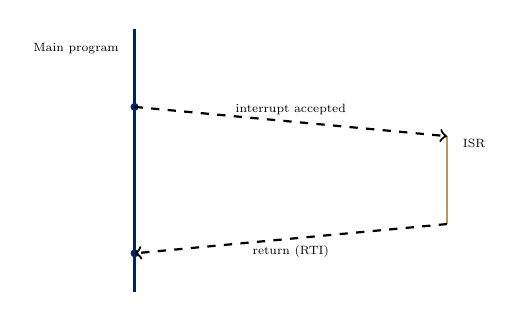
\begin{tikzpicture}[scale=0.62, transform shape,
      every node/.style={font=\small}]
    \draw[thick, primary-blue] (0,3.2) -- (0,-2.2);
    \node[font=\scriptsize, anchor=east] at (-0.2,2.8) {Main program};
    \draw[thick, primary-gold] (6.4,1.0) -- (6.4,-0.8);
    \node[font=\scriptsize, anchor=west] at (6.6,0.85) {ISR};
    \filldraw[primary-blue] (0,1.6) circle (2pt);
    \filldraw[primary-blue] (0,-1.4) circle (2pt);
    \draw[dashed, thick, ->] (0,1.6) -- (6.4,1.0)
          node[midway, above] {\scriptsize interrupt accepted};
    \draw[dashed, thick, ->] (6.4,-0.8) -- (0,-1.4)
          node[midway, below] {\scriptsize return (RTI)};
  \end{tikzpicture}
  \caption{Interrupt as a transfer of control: the main program is suspended when the interrupt is accepted, control jumps to the ISR, and \texttt{RTI} returns control to the main program exactly where it left off --- cf.\ Hamacher, \textit{Computer Organization and Embedded Systems}, 6th ed., Fig.~3.6, \S3.2, p.103--104 \cite{Hamacher2002_computer_organization}.}
  \label{fig:interrupt-transfer}
\end{figure}

\subsection{Enabling and Disabling Interrupts}

An interrupt request from a device does not automatically suspend the CPU; two independent switches must both agree before it is honored (Hamacher, 6th ed., \S3.2.1, p.106--107) \cite{Hamacher2002_computer_organization}:

\begin{itemize}
  \item \texttt{IE} --- a single interrupt-enable bit inside the processor status register (\texttt{PS}). When \texttt{IE}$=0$, the CPU ignores \emph{every} interrupt request, regardless of which device sent it.
  \item A per-device interrupt-enable bit inside that specific device's own control register --- \texttt{KIRQ} for the keyboard, \texttt{DIRQ} for the display. This bit controls whether \emph{this particular} device is allowed to request an interrupt at all.
\end{itemize}

A request reaches the CPU only when both switches agree: the device's own enable bit \emph{and} \texttt{PS.IE} must both be set. Plainly: \texttt{IE} is the master switch; each device also has its own little switch, and both must be on for the request to arrive. For example, \texttt{KIRQ}$=1$ and \texttt{IE}$=1$ means a keystroke will interrupt; \texttt{IE}$=0$ means it waits. This two-level gating means a programmer can globally mask all interrupts with one bit (useful, for instance, while updating shared data structures that an ISR must not see half-updated) while separately deciding, device by device, which sources are even allowed to ask.

\subsection{Worked Example: A Five-Step Interrupt-Handling Scenario}

\begin{example}[Handling One Keyboard Interrupt, Step by Step]
\label{ex:5step}
Hamacher's 6th edition works through interrupt handling as a five-step scenario (\S3.2.1, p.106--107) \cite{Hamacher2002_computer_organization}. Applying it concretely to the keyboard, with \texttt{KIRQ}$=1$ and \texttt{PS.IE}$=1$ already set:

\begin{enumerate}
  \item \textbf{Device signals readiness.} The keyboard sets its status flag \texttt{KIN}$=1$ in its status register, and because \texttt{KIRQ}$=1$, it also raises an interrupt-request line to the CPU.
  \item \textbf{CPU finishes what it was doing.} The CPU does not react mid-instruction; it always completes whatever instruction is currently executing first, then checks \texttt{PS.IE}.
  \item \textbf{CPU accepts the interrupt.} Since \texttt{PS.IE}$=1$, the CPU saves \texttt{PC} (and any registers the ISR is about to clobber) into shadow registers, clears \texttt{PS.IE} to 0 (so a second interrupt cannot interrupt this one, unless the ISR explicitly re-enables it), and loads \texttt{PC} with the keyboard ISR's starting address.
  \item \textbf{ISR services the device.} The keyboard ISR executes \texttt{MoveByte KBD\_DATA, R} to read the pending keystroke, which as a side effect clears \texttt{KIN} back to 0, and then executes a return-from-interrupt instruction.
  \item \textbf{Return-from-interrupt restores the original program.} \texttt{RTI} restores the saved \texttt{PC} from the shadow register and re-enables interrupts (\texttt{PS.IE}$\gets1$). The interrupted program resumes at exactly the instruction it would have executed next, with no memory of having been interrupted.
\end{enumerate}
Compared to Example~\ref{ex:polling}'s \texttt{READWAIT} loop, the CPU here does zero work while waiting for a keystroke --- it only spends time on the interrupt \emph{after} \texttt{KIN} actually becomes 1. The CPU never polls; it goes on computing until the device rings the bell.
\end{example}

\subsection{Handling Multiple Devices}

A single interrupt-request line tells the CPU \emph{that} something needs attention, but not \emph{which} device raised it. Hamacher's 6th edition presents two designs for resolving this (\S3.2.2, p.107--109) \cite{Hamacher2002_computer_organization}:

\begin{itemize}
  \item \textbf{Polling the sources.} On any interrupt, the ISR checks each device's status flag in turn, in some fixed order, until it finds the one that is set. This needs no extra hardware, but the fixed check order means dispatch time grows with the number of devices --- the last device checked pays the largest latency.
  \item \textbf{Vectored interrupts.} Each device supplies its own identifying code as part of the interrupt request. Hardware uses that code to index directly into an \textbf{interrupt-vector table} --- a table of ISR starting addresses, one entry per device --- and jumps straight to the correct ISR.
\end{itemize}

Vectored interrupts trade a small amount of extra hardware (the vector table itself, plus the lookup logic) for constant-time dispatch, regardless of how many devices are attached --- the CPU jumps directly to the right ISR instead of walking a checklist. Plainly: polling-the-sources asks everyone ``was it you?'' in order; a vector table skips the asking and goes straight to the right ISR.

\subsection{Interrupt Nesting and Priority}

When more than one device can interrupt, and interrupts can themselves be interrupted, the processor needs a systematic way to decide who goes first. Figure~\ref{fig:nesting} shows the register-level mechanism: each device's IRQ line feeds a bit inside \texttt{IPENDING}, a per-device interrupt-enable mask lives in \texttt{IENABLE}, and both converge on a priority encoder that, together with the vector-table lookup, produces the winning device's ISR starting address (Hamacher, 6th ed., \S3.2.4, Fig.~3.7, p.110--111) \cite{Hamacher2002_computer_organization}. This is the direct register-level analogue of Week 7's ``two sources feed \texttt{MPC}'' diagram: multiple candidate signals converge on one decision point.

\begin{figure}[h]
  \centering
  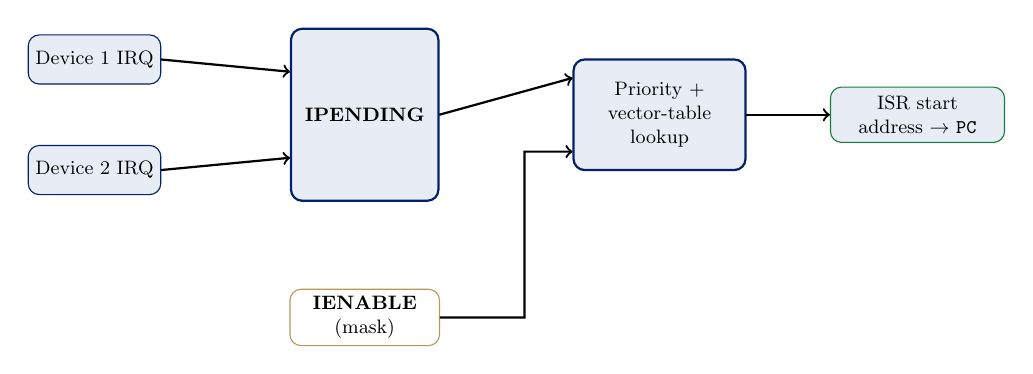
\begin{tikzpicture}[scale=0.78, transform shape,
      every node/.style={font=\small}]
    \node[draw=primary-blue, fill=light-bg, rounded corners,
          minimum width=2.0cm, minimum height=0.8cm, align=center]
          (D1) at (0,2.6) {Device 1 IRQ};
    \node[draw=primary-blue, fill=light-bg, rounded corners,
          minimum width=2.0cm, minimum height=0.8cm, align=center]
          (D2) at (0,0.8) {Device 2 IRQ};
    \node[draw=primary-blue, thick, fill=light-bg, rounded corners,
          minimum width=2.4cm, minimum height=2.8cm, align=center]
          (IPEND) at (4.4,1.7) {\textbf{IPENDING}};
    \node[draw=primary-gold, fill=white, rounded corners, text width=2.2cm,
          minimum height=0.9cm, align=center]
          (IENABLE) at (4.4,-1.6) {\textbf{IENABLE} (mask)};
    \node[draw=primary-blue, thick, fill=light-bg, rounded corners,
          minimum width=2.8cm, minimum height=1.8cm, align=center]
          (PRI) at (9.2,1.7) {Priority $+$\\vector-table\\lookup};
    \node[draw=positive, fill=light-bg, rounded corners, text width=2.6cm,
          minimum height=0.9cm, align=center]
          (OUT) at (13.4,1.7) {ISR start address $\to$ \texttt{PC}};
    \draw[->, thick] (D1.east) -- (IPEND.west |- 0,2.4);
    \draw[->, thick] (D2.east) -- (IPEND.west |- 0,1.0);
    \draw[->, thick] (IPEND.east) -- (PRI.west |- 0,2.3);
    \draw[->, thick] (IENABLE.east) -- (7.0,-1.6) -- (7.0,1.1) -- (PRI.west |- 0,1.1);
    \draw[->, thick] (PRI.east) -- (OUT.west);
  \end{tikzpicture}
  \caption{Interrupt dispatch with priority: device IRQ lines set bits in \texttt{IPENDING}; \texttt{IENABLE} masks which pending requests the priority encoder considers; the encoder plus vector-table lookup produces the winning ISR's starting address --- cf.\ Hamacher, \textit{Computer Organization and Embedded Systems}, 6th ed., Fig.~3.7, \S3.2.4, p.110--111 \cite{Hamacher2002_computer_organization}.}
  \label{fig:nesting}
\end{figure}

What the diagram shows: \texttt{IPENDING} latches \emph{which} devices currently want an interrupt; \texttt{IENABLE} decides \emph{which of those} are allowed through; the priority encoder picks the highest-priority allowed one; the vector table gives its ISR address. When two devices request simultaneously, the priority encoder grants the higher-priority one first; \texttt{IPENDING} keeps the other device's request latched --- not lost --- until that device is eventually serviced.

\begin{example}[Simultaneous Requests and Nesting]
\label{ex:nesting}
Device~1 has higher priority than Device~2. Both request an interrupt on the same cycle, and Device~1's ISR is still running when Device~2's request would otherwise be granted. Two cases follow directly from whether \emph{nesting} is enabled:
\begin{itemize}
  \item \textbf{Nesting allowed, and Device~2 outranks Device~1's ISR's running priority level.} Device~2 can interrupt Device~1's ISR itself --- the identical five-step scenario of Example~\ref{ex:5step} applies recursively, with Device~1's ISR now playing the role of the ``main program'' being suspended.
  \item \textbf{Nesting disabled, or Device~2 is lower priority than Device~1's currently-running ISR.} Device~2's request stays latched in \texttt{IPENDING}. It is not lost or re-requested; it simply waits until Device~1's ISR finishes and re-enables interrupts (\texttt{PS.IE}$\gets1$ via \texttt{RTI}), at which point the priority encoder re-evaluates \texttt{IPENDING} and grants Device~2.
\end{itemize}
\end{example}

\subsection{Exceptions: The General Form of an Interrupt}

The interrupt mechanism is not special to I/O devices; it is the same machinery the CPU uses for any event that must suspend the current program. Naming this generalization matters because it lets one mechanism serve many different sources.

\begin{definitionbox}{Exception}
An \textbf{exception} is any event that interrupts the normal flow of control --- an I/O interrupt, but also divide-by-zero, an illegal instruction, a page fault, or a timer tick. The interrupt mechanism is the same; only the \emph{source} differs (Hamacher, 6th ed., \S3.2.6, p.116--119; P\&H, ARM ed., Ch.~4, chapter-level) \cite{Hamacher2002_computer_organization,PattersonHennessy2017_computer_organization_design}.
\end{definitionbox}

Plainly, an interrupt is just one kind of exception --- the ``a device needs me'' kind. The CPU handles all of them with the same jump-to-handler machinery from Figure~\ref{fig:interrupt-transfer}: save state, service, restore. This is also the bridge later lectures will reuse --- exceptions are how the operating system gets control back from user programs.

Tracing one non-I/O exception through that machinery makes the generalization concrete, and shows exactly which step differs from an ordinary device interrupt.

\begin{example}[An Exception in Action: Divide-by-Zero]
\label{ex:exception-trace}
A running program executes \texttt{DIV R1, R2, R3} with \texttt{R3} holding \texttt{0}. No device is involved at all, yet the CPU services it with precisely the machinery built up in Section~\ref{sec:interrupts}:
\begin{enumerate}
  \item The ALU detects the divide-by-zero and raises a fixed \emph{internal} exception signal. There is no external device and no interrupt-request line --- the trigger originates inside the CPU itself.
  \item The CPU completes what it can of the current instruction and then forces a jump. This is the one step that differs from an ordinary interrupt: the jump is \emph{not} gated by \texttt{PS.IE}, because an exception of this kind cannot be masked. A program cannot elect to ignore its own divide-by-zero the way it can disable a keyboard interrupt.
  \item \texttt{PC} and the status register are saved into shadow registers, and \texttt{PC} is loaded with the fixed starting address of the divide-by-zero handler --- the same save-state step as Example~\ref{ex:5step}, reading a different entry of the same table.
  \item The handler runs (reporting the error, or handing control to the operating system), and the sequence closes with the same restore step an ISR uses.
\end{enumerate}
Same machinery, different trigger. A page fault, an illegal opcode, and a timer tick each follow this identical path, differing only in which starting address step 3 loads (Hamacher, 6th ed., \S3.2.6, p.116--119; P\&H, ARM ed., Ch.~4, chapter-level) \cite{Hamacher2002_computer_organization,PattersonHennessy2017_computer_organization_design}.
\end{example}

\subsection{Polling vs.\ Interrupts: Trade-offs}

\begin{center}
\footnotesize
\begin{tabular}{@{}lll@{}}
\toprule
& \textbf{Polling} & \textbf{Interrupts} \\
\midrule
Who initiates & CPU (asks repeatedly) & Device (signals once, when ready) \\
CPU cost while waiting & Wasted spin cycles & Zero --- CPU runs other code \\
Extra hardware & None & \texttt{IE}, per-device enables, vector table \\
Response latency & Depends on poll rate & Interrupt latency (usually smaller) \\
Best fit & One slow device, nothing else to do & Multiple/unpredictable devices \\
\bottomrule
\end{tabular}
\end{center}

Both techniques solve the same problem --- \emph{someone} has to notice when a device is ready --- but move the initiative in opposite directions. Interrupts do not eliminate the waiting cost; they relocate it from wasted CPU cycles to the hardware that detects readiness and raises the request line.

\section{The Hardware View: Synchronous and Asynchronous Bus Protocols}
\label{sec:bus}

Sections~\ref{sec:polling}--\ref{sec:interrupts} took the device interface for granted and asked only \emph{when} the CPU checks or is notified. This section drops one level, to the wires themselves: when a device interface says ``I'm not ready yet'' or ``here is the data,'' how is that actually communicated on the bus?

\subsection{Bus Structure: Master and Slave Roles}

Every I/O interface in Figure~\ref{fig:device-interface} in fact hangs off a single shared \textbf{bus} --- a set of address, data, and control lines that every attached device listens to (Hamacher, 6th ed., \S7.1, Fig.~7.1--7.2, p.228) \cite{Hamacher2002_computer_organization}. A \textbf{bus protocol} defines how a \textbf{master} (the device driving the transfer --- usually the CPU) and a \textbf{slave} (the device responding to it) coordinate a single data transfer without colliding. This section's question is: when a master says ``take this data'' or ``give me that data,'' how does the slave say ``I'm not ready yet'' or ``here it is''? Two different answers exist: \textbf{synchronous} and \textbf{asynchronous} bus protocols (Hamacher, 6th ed., \S7.2, p.229) \cite{Hamacher2002_computer_organization}.

\subsection{Synchronous Bus}

\begin{definitionbox}{Synchronous Bus}
On a \textbf{synchronous bus}, all devices share a common \textbf{bus clock}. The master places an address/data value on the bus at a fixed clock edge; every slave samples the bus at that \emph{same} edge, with no per-transfer negotiation (Hamacher, 6th ed., \S7.2.1, p.230--233) \cite{Hamacher2002_computer_organization}.
\end{definitionbox}

Figure~\ref{fig:sync-bus} shows the timing diagram for a synchronous transfer that must wait on a slow slave. Three signals run in parallel over time: the shared clock, the address/data lines (held valid across the whole transfer), and a \texttt{Slave-ready} line that stays low --- meaning ``not yet'' --- for as many extra clock cycles as the slow device needs, then rises once the data is actually valid.

\begin{figure}[h]
  \centering
  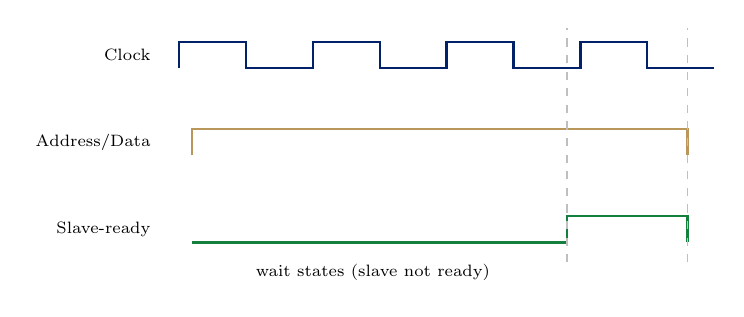
\begin{tikzpicture}[scale=0.85, transform shape,
      every node/.style={font=\scriptsize}]
    \node[anchor=east] at (-0.3,2.6) {Clock};
    \draw[thick, primary-blue]
      (0,2.4) -- (0,2.8) -- (1,2.8) -- (1,2.4) -- (2,2.4) -- (2,2.8) --
      (3,2.8) -- (3,2.4) -- (4,2.4) -- (4,2.8) -- (5,2.8) -- (5,2.4) --
      (6,2.4) -- (6,2.8) -- (7,2.8) -- (7,2.4) -- (8,2.4);
    \node[anchor=east] at (-0.3,1.3) {Address/Data};
    \draw[thick, primary-gold]
      (0.2,1.1) -- (0.2,1.5) -- (7.6,1.5) -- (7.6,1.1);
    \node[anchor=east] at (-0.3,0) {Slave-ready};
    \draw[thick, positive]
      (0.2,-0.2) -- (5.8,-0.2) -- (5.8,0.2) -- (7.6,0.2) -- (7.6,-0.2);
    \node[font=\scriptsize] at (2.9,-0.65) {wait states (slave not ready)};
    \draw[dashed, gray!50] (5.8,-0.5) -- (5.8,3.0);
    \draw[dashed, gray!50] (7.6,-0.5) -- (7.6,3.0);
  \end{tikzpicture}
  \caption{Synchronous-bus timing with wait states: the address/data lines are held valid across the whole transfer while \texttt{Slave-ready} stays low for several extra clock periods until the slow slave is finally ready --- cf.\ Hamacher, \textit{Computer Organization and Embedded Systems}, 6th ed., Fig.~7.3--7.5, \S7.2.1, p.230--233 \cite{Hamacher2002_computer_organization}.}
  \label{fig:sync-bus}
\end{figure}

\begin{example}[Reading the Synchronous-Bus Wait-State Timeline]
\label{ex:sync-trace}
Following Figure~\ref{fig:sync-bus} left to right against the running 4096-byte block-transfer example: at the first clock edge (time 0), the master places the target address on the address/data lines and they remain valid there for the rest of the diagram. \texttt{Slave-ready} starts low, meaning the slave has not yet placed (or accepted) valid data. For several full clock periods --- the ``wait states'' region --- the clock continues to toggle every half-period, but \texttt{Slave-ready} stays low each time, because the slow device physically has not finished. Only at the clock edge marked by the first dashed vertical line does \texttt{Slave-ready} finally rise; the master samples the bus at the \emph{next} clock edge (the second dashed line) and the transfer of that one word completes. A fast device would need zero wait states --- \texttt{Slave-ready} would already be high at the very first edge --- while a slower device simply holds \texttt{Slave-ready} low for as many extra clock cycles as it needs; the master's logic does not otherwise change.
\end{example}

The timeline above is qualitative --- ``several'' wait states. Putting a device speed and a clock rate on it turns the picture into a number, and shows how directly the wait-state count follows from the mismatch between the two.

\begin{example}[How Many Wait States Does a Slow Device Cost?]
\label{ex:wait-states}
Take the running block transfer's disk controller, and suppose it needs 100~ns to place a word on the bus. The synchronous bus clock runs at 500~MHz. How many wait states does the master insert for one word?

The clock period is $1/(500 \times 10^6) = 2$~ns. Covering the disk's 100~ns response therefore takes
\[
  \frac{100~\text{ns}}{2~\text{ns/cycle}} = 50 \text{ clock cycles.}
\]
One of those 50 is the ``normal'' data cycle the transfer would have needed even from an instantly-ready device, so the master inserts \textbf{49 wait-state cycles}: the slave holds \texttt{Slave-ready} low for all 49, exactly as in the wait-state region of Figure~\ref{fig:sync-bus}, and the transfer completes on the 50th.

The comparison with Section~\ref{sec:polling} is worth drawing explicitly. Example~\ref{ex:polling-waste} found roughly $2\times10^8$ wasted polls for a single keystroke; here a slow device costs 49 idle bus cycles per word. A slow device is expensive under \emph{every} technique in this chapter --- what changes between techniques is only \emph{who} pays the cost and \emph{how much} of the CPU it consumes.
\end{example}

\subsection{Asynchronous Bus (Full Handshake)}

\begin{definitionbox}{Asynchronous Bus (Full Handshake)}
An \textbf{asynchronous bus} has no shared clock. Master and slave exchange explicit \textbf{Master-ready}/\textbf{Slave-ready} signals, each one changing only \emph{in response to} the other --- a \textbf{full handshake} (Hamacher, 6th ed., \S7.2.2, p.233--236) \cite{Hamacher2002_computer_organization}.
\end{definitionbox}

Figure~\ref{fig:async-bus} shows this exchange as a four-step interlocked ladder between a Master column and a Slave column, where each arrow only fires after the previous one has been observed.

\begin{figure}[h]
  \centering
  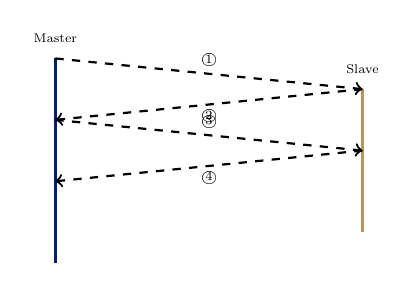
\begin{tikzpicture}[scale=0.65, transform shape,
      every node/.style={font=\small}]
    \node[font=\scriptsize] at (0,4.0) {Master};
    \node[font=\scriptsize] at (6.0,3.4) {Slave};
    \draw[thick, primary-blue] (0,3.6) -- (0,-0.4);
    \draw[thick, primary-gold] (6.0,3.0) -- (6.0,0.2);
    \draw[dashed, thick, ->] (0,3.6) -- (6.0,3.0)
          node[midway, above] {\scriptsize \textcircled{\scriptsize 1}};
    \draw[dashed, thick, ->] (6.0,3.0) -- (0,2.4)
          node[midway, below] {\scriptsize \textcircled{\scriptsize 2}};
    \draw[dashed, thick, ->] (0,2.4) -- (6.0,1.8)
          node[midway, above] {\scriptsize \textcircled{\scriptsize 3}};
    \draw[dashed, thick, ->] (6.0,1.8) -- (0,1.2)
          node[midway, below] {\scriptsize \textcircled{\scriptsize 4}};
  \end{tikzpicture}
  \caption{The asynchronous full handshake as a four-step interlocked exchange between master and slave --- cf.\ Hamacher, \textit{Computer Organization and Embedded Systems}, 6th ed., Fig.~7.6--7.7, \S7.2.2, p.233--236 \cite{Hamacher2002_computer_organization}.}
  \label{fig:async-bus}
\end{figure}

\begin{center}
\footnotesize
\begin{tabular}{@{}p{0.46\textwidth}p{0.46\textwidth}@{}}
  \textcircled{\scriptsize 1} Master-ready asserted &
  \textcircled{\scriptsize 2} Slave-ready (data valid) \\
  \textcircled{\scriptsize 3} Master-ready withdrawn (latched) &
  \textcircled{\scriptsize 4} Slave-ready withdrawn \\
\end{tabular}
\end{center}

\begin{example}[Walking the Four-Step Handshake]
\label{ex:async-trace}
Applying the four steps of Figure~\ref{fig:async-bus} to one word of the running 4096-byte block transfer, in strict sequence, with each step waiting for the previous one to be observed before it can fire:
\begin{enumerate}
  \item \textbf{Master-ready asserted.} The master places the address/data on the bus and asserts \texttt{Master-ready}, announcing ``I have placed a value; take it (or: I am ready to receive).''
  \item \textbf{Slave-ready (data valid).} Only after observing \texttt{Master-ready}, the slave completes its side of the transfer (latching the data, or supplying it) and asserts \texttt{Slave-ready}, announcing ``done, data is valid.''
  \item \textbf{Master-ready withdrawn (latched).} Only after observing \texttt{Slave-ready}, the master withdraws \texttt{Master-ready} --- it has now recorded that the transfer completed.
  \item \textbf{Slave-ready withdrawn.} Only after observing \texttt{Master-ready} drop, the slave withdraws \texttt{Slave-ready}, returning both lines to their idle state and readying the bus for the next word.
\end{enumerate}
Because each step is triggered only by observing the previous one --- never by a shared clock edge --- \textbf{bus skew} (different wires physically arriving at slightly different times) never causes a false sample: a device simply waits until it actually observes the other side's signal, however long that takes. This is the crucial difference from Figure~\ref{fig:sync-bus}'s synchronous protocol, where every device must sample at the same fixed clock edge regardless of individual wire delays.
\end{example}

\subsection{Synchronous vs.\ Asynchronous: Trade-offs}

\begin{center}
\footnotesize
\begin{tabular}{@{}lll@{}}
\toprule
& \textbf{Synchronous} & \textbf{Asynchronous} \\
\midrule
Timing reference & Shared bus clock & Explicit handshake, no clock \\
Slow-device handling & Extra wait-state clock cycles & Handshake simply takes longer \\
Skew sensitivity & Sensitive --- must beat clock period & Immune --- self-timed \\
Per-transfer overhead & Low (one clock edge) & Higher (two round trips) \\
Best fit & Devices of similar, known speed & Mixed-speed / unpredictable devices \\
\bottomrule
\end{tabular}
\end{center}

Both protocols solve the identical coordination problem --- ``how does the slave say it's ready?'' --- but with opposite mechanisms: a shared clock that every device trusts implicitly, versus an explicit conversation that assumes nothing about timing at all.

\begin{example}[Why Not Always Use Asynchronous?]
\label{ex:why-sync}
Asynchronous handshaking tolerates skew and adapts automatically to any device speed, which sounds strictly better --- so why do most high-speed processor buses use synchronous protocols instead? The answer is in the ``per-transfer overhead'' row of the trade-off table above: every asynchronous transfer pays \emph{two full round-trip delays} --- steps 1--2 of Example~\ref{ex:async-trace} form one round trip, and steps 3--4 form a second. For a device that is consistently fast, both round trips are pure overhead that a synchronous bus never pays; the synchronous bus only loses ground when a device is unusually slow (extra wait states, as in Example~\ref{ex:sync-trace}) or when the clock period must shrink to accommodate skew across many devices. High-speed buses connecting devices of known, similar speed --- exactly the synchronous bus's ``best fit'' row --- therefore favor the cheaper synchronous protocol.
\end{example}

\section{Direct Memory Access and I/O Processors}
\label{sec:dma}

\subsection{The Cost Interrupts Still Pay}

Interrupts (Section~\ref{sec:interrupts}) removed the CPU's \emph{waiting} cost, but not its \emph{involvement} in actually moving data. This is easiest to see by returning to the running 4096-byte block-transfer example and asking what interrupt-driven I/O costs when the transfer is one word at a time, four bytes per word.

\begin{example}[Counting ISR Invocations for a Block Transfer]
\label{ex:isr-count}
With interrupt-driven I/O, the ISR from Example~\ref{ex:5step} executes once per word: read status, read/write data, update a memory pointer, decrement a word counter, and return. A 4096-byte disk transfer, moved four bytes at a time, therefore requires
\[
4096 \div 4 = 1024
\]
separate ISR invocations for a \emph{single} block transfer. Interrupts eliminated the CPU spinning idly between words, but the CPU is still fully engaged for all 1024 of those short ISR executions --- one context switch into the ISR and back out, per word. The next technique removes the CPU from the data-movement path itself.
\end{example}

\subsection{Bus Arbitration: A Third Role for a Device}

DMA depends on a capability not yet introduced: an I/O device, not just the CPU, becoming bus master. \textbf{Bus arbitration} is the mechanism that decides which of several candidate masters gets the bus on any given cycle (Hamacher, 6th ed., \S7.3, Fig.~7.8--7.9, p.237--238) \cite{Hamacher2002_computer_organization}. Figure~\ref{fig:arbitration} shows three candidate masters, each able to assert a bus-request line (\texttt{BR}), feeding into an arbiter; the arbiter grants the bus to exactly one requester at a time, by priority, over a bus-grant line (\texttt{BG}).

\begin{figure}[h]
  \centering
  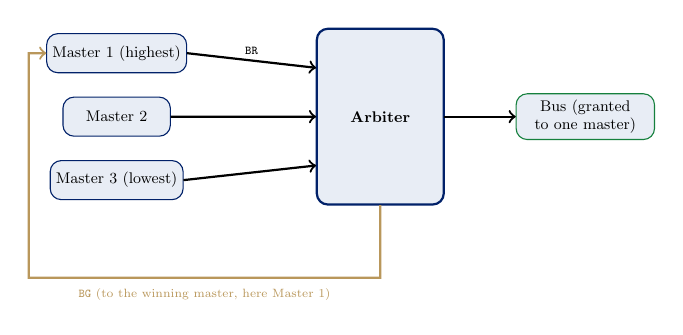
\begin{tikzpicture}[scale=0.62, transform shape,
      every node/.style={font=\small}]
    \node[draw=primary-blue, fill=light-bg, rounded corners,
          minimum width=2.2cm, minimum height=0.8cm, align=center]
          (M1) at (0,2.6) {Master 1 (highest)};
    \node[draw=primary-blue, fill=light-bg, rounded corners,
          minimum width=2.2cm, minimum height=0.8cm, align=center]
          (M2) at (0,1.3) {Master 2};
    \node[draw=primary-blue, fill=light-bg, rounded corners,
          minimum width=2.2cm, minimum height=0.8cm, align=center]
          (M3) at (0,0) {Master 3 (lowest)};
    \node[draw=primary-blue, thick, fill=light-bg, rounded corners,
          minimum width=2.6cm, minimum height=3.6cm, align=center]
          (ARB) at (5.4,1.3) {\textbf{Arbiter}};
    \node[draw=positive, fill=light-bg, rounded corners, text width=2.6cm,
          minimum height=0.9cm, align=center]
          (BUS) at (9.6,1.3) {Bus (granted to one master)};
    \draw[->, thick] (M1.east) -- (ARB.west |- 0,2.3)
          node[midway, above] {\scriptsize \texttt{BR}};
    \draw[->, thick] (M2.east) -- (ARB.west |- 0,1.3);
    \draw[->, thick] (M3.east) -- (ARB.west |- 0,0.3);
    \draw[->, thick, primary-gold] (ARB.south) -- (5.4,-2.0) -- (-1.8,-2.0) -- (-1.8,2.6) -- (M1.west);
    \node[font=\scriptsize, primary-gold] at (1.8,-2.35)
          {\texttt{BG} (to the winning master, here Master 1)};
    \draw[->, thick] (ARB.east) -- (BUS.west);
  \end{tikzpicture}
  \caption{Bus arbitration: three candidate masters assert \texttt{BR}; the arbiter grants \texttt{BG} to exactly one requester, by priority, at a time --- cf.\ Hamacher, \textit{Computer Organization and Embedded Systems}, 6th ed., Fig.~7.8--7.9, \S7.3, p.237--238 \cite{Hamacher2002_computer_organization}.}
  \label{fig:arbitration}
\end{figure}

\begin{example}[Three-Master Priority Arbitration]
\label{ex:arbitration}
Suppose Masters~1, 2, and~3 (priority highest to lowest, as in Figure~\ref{fig:arbitration}) all assert \texttt{BR} on the same cycle, competing for the bus. The arbiter examines all three requests simultaneously and grants \texttt{BG} to Master~1, the highest-priority requester --- Masters~2 and~3 continue holding \texttt{BR} asserted, waiting. Once Master~1 finishes its transfer and releases the bus, the arbiter re-evaluates the still-pending requests from Masters~2 and~3 and grants \texttt{BG} to Master~2 next, by the same priority rule; Master~3 is served last, once both higher-priority masters have released the bus. Any device wired into the \texttt{BR}/\texttt{BG} scheme can become bus master this way --- not only the CPU --- which is exactly the capability DMA needs. Being bus master is how a device talks to memory \emph{directly}.
\end{example}

\subsection{From Arbitration to Direct Memory Access}

Once a device can become bus master via arbitration, it can transfer data \emph{directly to or from memory}, with no CPU instruction ever touching the data. The CPU is interrupted only \emph{once}, when the entire block finishes, not once per word as in Example~\ref{ex:isr-count}. This edition of Hamacher's text describes exactly this mechanism in \S7.3 (Arbitration) but never names it ``DMA'' --- the term and its standard treatment below follow Stallings Ch.~8, per the syllabus and the project's textbook-grounding rule, since this book's index does not cover DMA/IOP by name \cite{Hamacher2002_computer_organization}.

\begin{definitionbox}{Direct Memory Access (DMA) --- general/standard treatment, Stallings Ch.~8}
A \textbf{DMA controller} is given a source/destination address and a word count by the CPU, then becomes bus master (via the arbitration mechanism of Figure~\ref{fig:arbitration}) and transfers the entire block directly to/from memory, interrupting the CPU only when the \emph{block} --- not each word --- is complete \cite{Stallings2015_computer_organization}.
\end{definitionbox}

Plainly: the CPU says ``copy this block,'' then goes back to work; the DMA controller does the copying and rings the bell when done.

\subsection{The DMA Controller: What's Inside}

To do its job, the DMA controller carries four registers, all written once by the CPU at setup and owned by the controller for the rest of the transfer. Figure~\ref{fig:dma-regs} shows where they live: the DMA controller sits between the CPU and the I/O device on the bus, and can become bus master to reach memory directly.

\begin{figure}[h]
  \centering
  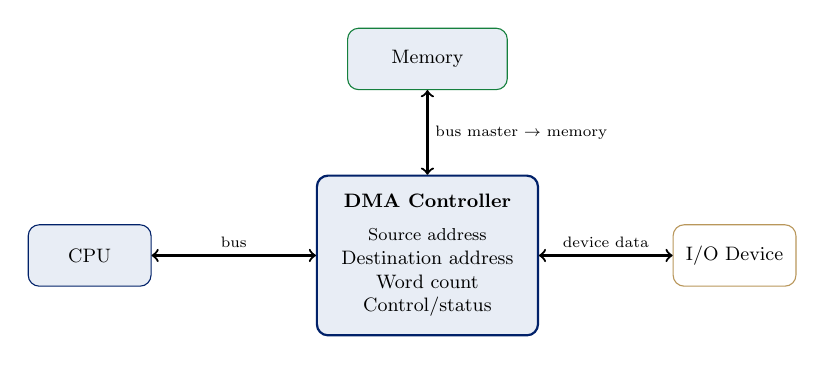
\begin{tikzpicture}[scale=0.78, transform shape,
      every node/.style={font=\small}]
    \node[draw=primary-blue, fill=light-bg, rounded corners,
          minimum width=2.0cm, minimum height=1.0cm, align=center]
          (CPU) at (0,0) {CPU};
    \node[draw=primary-blue, thick, fill=light-bg, rounded corners,
          minimum width=3.6cm, minimum height=2.6cm, align=center]
          (DMA) at (5.5,0) {\textbf{DMA Controller}\\[0.15cm]
            \footnotesize
            Source address\\ Destination address\\ Word count\\
            Control/status};
    \node[draw=primary-gold, fill=white, rounded corners,
          minimum width=2.0cm, minimum height=1.0cm, align=center]
          (DEV) at (10.5,0) {I/O Device};
    \node[draw=positive, fill=light-bg, rounded corners,
          minimum width=2.6cm, minimum height=1.0cm, align=center]
          (MEM) at (5.5,3.2) {Memory};
    \draw[<->, thick] (CPU.east) -- (DMA.west)
          node[midway, above] {\scriptsize bus};
    \draw[<->, thick] (DMA.east) -- (DEV.west)
          node[midway, above] {\scriptsize device data};
    \draw[<->, thick] (DMA.north) -- (MEM.south)
          node[midway, right] {\scriptsize bus master $\to$ memory};
  \end{tikzpicture}
  \caption{The DMA controller and its four registers: source/destination address, word count, and control/status. The CPU writes them once at setup; the controller becomes bus master to move data directly between the device and memory --- general/standard treatment, Stallings Ch.~8 \cite{Stallings2015_computer_organization}.}
  \label{fig:dma-regs}
\end{figure}

\begin{itemize}
  \item \textbf{Source / destination address} --- where the data comes from and goes to (memory address and device, or vice versa).
  \item \textbf{Word count} --- how many words remain to transfer; decremented after every word.
  \item \textbf{Control/status} --- transfer direction, mode, and the ``block done'' flag that interrupts the CPU.
\end{itemize}

\subsection{How a DMA Transfer Runs: Step by Step}

\begin{example}[The Six-Step DMA Transfer Sequence]
\label{ex:dma-seq}
Copying the running 4096-byte block from disk to memory, the CPU appears exactly twice --- at setup and at completion --- and never touches the data itself \cite{Stallings2015_computer_organization}:
\begin{enumerate}
  \item \textbf{Setup.} The CPU writes the DMA controller's registers: source address (disk), destination address (memory), word count (1024), and direction (read).
  \item \textbf{Request.} The DMA controller asks for the bus by asserting \texttt{BR} (bus request).
  \item \textbf{Grant.} The arbiter answers with \texttt{BG} (bus grant); the DMA controller becomes bus master (Hamacher, 6th ed., \S7.3, p.237--238) \cite{Hamacher2002_computer_organization}.
  \item \textbf{Transfer one word.} The DMA controller reads one word from the device and writes it to memory (or the reverse), using one or two bus cycles.
  \item \textbf{Decrement.} It subtracts 1 from the word count and, if the count is still $>0$, returns to step 2 for the next word.
  \item \textbf{Done.} When the count reaches 0, the DMA controller drops \texttt{BR} and raises a \emph{completion interrupt} --- the CPU's only involvement after setup.
\end{enumerate}
Compare with polling and interrupts: the CPU now appears exactly twice, at the start and the end.
\end{example}

\subsection{DMA Transfer Modes}

The DMA controller can choose how aggressively it holds the bus. The trade-off is always the same --- speed of the transfer versus how much it starves the CPU --- and three standard modes span the range (general/standard treatment, Stallings Ch.~8) \cite{Stallings2015_computer_organization}:

\begin{description}
  \item[\textbf{Burst (block) mode.}] The DMA controller holds the bus for the \emph{entire} block --- all 1024 words in one continuous burst, then releases the bus and interrupts the CPU. Fastest possible block transfer, but the CPU cannot reach memory at all for the duration of the burst.
  \item[\textbf{Cycle-stealing (single) mode.}] The DMA controller grabs the bus for \emph{one word}, releases it, and re-requests --- so the CPU can use the bus between DMA words. Slower per block, but the CPU keeps running between transfers.
  \item[\textbf{Transparent (hidden) mode.}] The DMA controller transfers \emph{only during CPU cycles that do not use the bus at all} --- the CPU never even notices the DMA happening. Slowest transfer rate, but zero effect on the CPU.
\end{description}

Plainly: burst = ``whole job now, don't bother me''; cycle stealing = ``one word, then back off''; transparent = ``only when you're not looking.''

\begin{center}
\footnotesize
\begin{tabular}{@{}llll@{}}
\toprule
& \textbf{Burst} & \textbf{Cycle stealing} & \textbf{Transparent} \\
\midrule
Bus held & Whole block & One word & Only idle CPU cycles \\
Transfer speed & Fastest & Medium & Slowest \\
Effect on CPU & Starved for the block & Brief pauses per word & None \\
\bottomrule
\end{tabular}
\end{center}

\subsection{DMA's Cost Reduction on the Running Block Transfer}

\begin{example}[DMA's Cost Reduction on the Running Block Transfer]
\label{ex:dma-cost}
Revisiting Example~\ref{ex:isr-count}'s 4096-byte transfer under DMA: the CPU's only involvement is a single setup step (write the source/destination address and the word count of 1024 into the DMA controller's registers) and a single completion interrupt once the DMA controller has moved all 1024 words. This is a reduction from 1024 ISR invocations to 2 CPU events total (1 setup $+$ 1 completion interrupt) --- a constant cost regardless of block size, in contrast to interrupt-driven I/O's cost, which grows linearly with the number of words transferred.

Putting instruction counts on it makes the saving concrete: if one ISR takes 200 CPU instructions, interrupt-driven I/O spends $1024\times200 = 204{,}800$ instructions moving the block, while DMA spends one setup plus one completion ISR --- roughly 400 instructions --- about \emph{500$\times$ less} CPU work. The CPU that used to spend its whole time servicing the disk can now run the user's program instead.

The trade-off is that the DMA controller and the CPU now compete for the same memory bus while the transfer is in progress (the bus is occupied for the same 1024 transfer cycles either way), and a physical DMA controller is extra hardware neither polling nor plain interrupts require.
\end{example}

\subsection{I/O Processors (IOP)}

\begin{definitionbox}{I/O Processor (IOP) --- general/standard treatment, Stallings Ch.~8}
An \textbf{I/O processor} generalizes DMA one step further: a dedicated processor, given a whole \emph{channel program} (a short program describing several transfers, data formats, and simple decisions), executes it independently --- interrupting the main CPU only when the \emph{entire program} completes, not per block \cite{Stallings2015_computer_organization}.
\end{definitionbox}

Plainly: DMA copies one block; an IOP runs a whole to-do list of I/O jobs and reports back when the list is done. Where DMA offloads only the \emph{moving} of data, an IOP offloads \emph{managing a sequence} of I/O operations. The distinction is how much decision-making is delegated away from the main CPU, not merely how the data physically moves: a DMA controller executes one pre-configured block transfer and stops; an IOP can execute a whole program of transfers, formats, and conditional decisions on its own, reporting back to the CPU only when that entire program is done.

What a channel program actually looks like is easiest to see on a job that chains several unlike operations together.

\begin{example}[A Channel Program for an IOP]
\label{ex:channel-program}
A print job needs three things done in order: read a 4096-byte record from disk, convert it to the printer's character format, and send it to the printer --- with the CPU interrupted only once, when all three have finished.
\begin{enumerate}
  \item \textbf{Setup.} The CPU writes a short channel program into memory --- three steps, \texttt{READ disk} $\to$ \texttt{buffer}, \texttt{CONVERT buffer} $\to$ \texttt{buffer2}, \texttt{WRITE buffer2} $\to$ \texttt{printer} --- and hands the IOP that program's starting address.
  \item \textbf{Execution.} The IOP runs all three steps itself, becoming bus master as needed by exactly the arbitration mechanism of Section~\ref{sec:dma}, with no CPU involvement between steps.
  \item \textbf{Completion.} Only once the \texttt{WRITE} step finishes does the IOP raise a single interrupt. The CPU never observes the intermediate \texttt{READ} and \texttt{CONVERT} steps at all.
\end{enumerate}
The contrast with DMA is the point. A DMA controller's ``program'' is always the same single step --- copy this block --- so a job like this one would cost the CPU three separate setup-and-completion cycles, one per operation. An IOP's channel program chains several \emph{different} operations, including a format conversion that is not a data transfer at all, which is precisely the additional delegation described in Stallings Ch.~8 (general/standard treatment) \cite{Stallings2015_computer_organization}.
\end{example}

\subsection{Four I/O Techniques, Head to Head}

\begin{center}
\tiny
\begin{tabular}{@{}lllll@{}}
\toprule
& \textbf{Polling} & \textbf{Interrupts} & \textbf{DMA} & \textbf{IOP} \\
\midrule
CPU cost / word & Every poll & Every word (ISR) & None (setup only) & None \\
CPU cost / block & --- & Thousands of ISRs & One interrupt & One interrupt \\
Extra hardware & None & Vector table, \texttt{IE} & DMA controller & Dedicated processor \\
Best fit & One slow device & Multiple/sporadic devices & Bulk block transfer & Complex I/O subsystems \\
\bottomrule
\end{tabular}
\end{center}

All four techniques answer the same core question --- who watches the device, and how much of the CPU does watching cost? --- with a monotonically decreasing amount of CPU involvement, purchased with a monotonically increasing amount of dedicated hardware.

\begin{example}[Choosing a Technique for Two Different Devices]
\label{ex:choosing}
A system reads one temperature-sensor value per second (a low rate, and the application can tolerate some latency in reading it) and, separately, copies a 10~MB file from disk to memory (a high rate, throughput-critical operation). Applying the head-to-head comparison above to each:
\begin{itemize}
  \item \textbf{Temperature sensor: interrupts.} At one event per second, the ISR overhead per event (a handful of instructions, per Example~\ref{ex:5step}) is utterly negligible relative to the CPU's billions of instructions per second, and the CPU remains completely free to do other work the rest of the time. Polling would waste cycles for no benefit (as in Example~\ref{ex:polling-waste}); DMA/IOP hardware would be pure overkill for a single value per second.
  \item \textbf{Disk copy: DMA.} At 10~MB moved in 4-byte words, interrupt-driven I/O would need on the order of $2.5\times10^6$ ISR invocations (following the arithmetic of Example~\ref{ex:isr-count} scaled up), which would dominate CPU time entirely. DMA reduces the CPU's involvement to one setup and one completion interrupt regardless of the block's size, exactly the trade-off Example~\ref{ex:dma-cost} quantified.
\end{itemize}
The rule of thumb: match the technique to the \emph{rate} and \emph{size} of the transfer, not to habit.
\end{example}

\section{Synthesis: The Four Threads Meet}
\label{sec:synthesis}

Every design decision in this chapter moves the cost of ``someone has to notice the device is ready, and someone has to move the data'' to a different place --- CPU cycles, dedicated hardware, or per-transfer wire delay --- never eliminating it outright.

\textbf{Polling vs.\ interrupts} (the programmer's view, Sections~\ref{sec:polling}--\ref{sec:interrupts}): polling wastes CPU cycles asking a status flag that has not changed; interrupts let the device ask instead, at the cost of the vector-table and priority hardware from Figure~\ref{fig:nesting}.

\textbf{Synchronous vs.\ asynchronous} (the bus hardware, Section~\ref{sec:bus}): a shared clock is cheap per transfer but sensitive to skew and slow devices (Figure~\ref{fig:sync-bus}); an explicit handshake is skew-immune but pays two full round trips on every single transfer (Figure~\ref{fig:async-bus}).

\textbf{Interrupts vs.\ DMA/IOP} (who actually moves the data, Section~\ref{sec:dma}): interrupts still touch every single word (Example~\ref{ex:isr-count}); DMA and IOP remove the CPU from the data path entirely, trading extra hardware (a DMA controller, or a whole dedicated processor) for near-zero per-word CPU cost (Example~\ref{ex:dma-cost}).

None of these three trade-offs is free --- exactly the pattern Weeks 5--7 already established for bus organization and control-unit design, now applied to the world outside the chip rather than inside it.

Weeks 1--8 together built a CPU that computes, controls itself, and now moves data to and from slow external devices. Week 9 asks the next question in the same speed-mismatch pattern: once data is in memory, how do we make \emph{memory itself} fast enough to keep up with the CPU? DRAM is far slower than the CPU, reproducing the identical speed-mismatch problem this chapter solved for I/O devices, but for memory instead --- cache memory, mapping functions, and replacement policies are Week 9's answer.

\subsection{Summary}

\textbf{Memory-mapped I/O} places a device's data/status/control registers directly in the normal address space (the \textbf{isolated-I/O} alternative needs separate I/O instructions and a separate address space); \textbf{program-controlled I/O (polling)} repeatedly tests a status flag (\texttt{KIN}, \texttt{DOUT}) until it changes. \textbf{Interrupts} let the device signal readiness instead: \texttt{PS.IE} and per-device enables (\texttt{KIRQ}/\texttt{DIRQ}) gate delivery, and \textbf{vectored interrupts} use \texttt{IPENDING}/\texttt{IENABLE} plus an interrupt-vector table for constant-time dispatch regardless of device count; an \textbf{exception} generalizes the same mechanism to non-I/O events. On the hardware side, a \textbf{synchronous bus} uses a shared clock and wait states for slow slaves, while an \textbf{asynchronous bus} uses a \texttt{Master-ready}/\texttt{Slave-ready} full handshake --- skew-immune, but at a higher per-transfer overhead of two round trips. \textbf{Bus arbitration} (\texttt{BR}/\texttt{BG}) lets any device become bus master, which is the functional basis for \textbf{DMA} --- a controller with source/destination address, word count, and control/status registers, running a six-step transfer in burst, cycle-stealing, or transparent mode, one setup plus one block-completion interrupt --- and the \textbf{IOP} (a whole channel program executed independently, general/standard treatment per Stallings Ch.~8). All four techniques answer the same underlying question --- how much of the CPU does watching and moving the data cost, and how much hardware buys that cost down?

\subsection*{Exercises}

\begin{enumerate}
  \item A printer produces output slowly enough that the CPU can service it with either polling or interrupts. Explain, using the reasoning of Example~\ref{ex:polling-waste}, why interrupts become strictly preferable as the CPU's clock rate increases relative to the printer's fixed speed, even though the printer's own speed never changes.
  \item Extend Example~\ref{ex:5step}'s five-step scenario to a \emph{second} interrupt-capable device, a mouse, with lower priority than the keyboard and \texttt{PS.IE} initially $=1$. Write out, step by step, what happens if the mouse raises an interrupt request while the keyboard's ISR is already running and interrupt nesting is disabled.
  \item A synchronous bus transfer (as in Figure~\ref{fig:sync-bus}) needs 3 wait-state clock cycles at a 200~MHz bus clock before \texttt{Slave-ready} rises. Compute the total time, in nanoseconds, from the first clock edge until the transfer completes (the edge at which the master samples valid data), counting the wait states plus the one clock period needed to actually sample.
  \item Following Example~\ref{ex:arbitration}, suppose a fourth master (lowest priority, below Master~3) also asserts \texttt{BR} on the same cycle as Masters~1--3. In what order are all four masters granted the bus, assuming each releases the bus promptly after its own transfer and no new requests arrive in the meantime?
  \item Using Example~\ref{ex:dma-cost}'s method, compute the number of ISR invocations interrupt-driven I/O would need, and the number of CPU events DMA would need, to transfer an 8192-byte block, again 4 bytes per word. Compare the two totals and state, in one sentence, which technique's cost is scale-independent and which is not.
  \item A DMA controller is configured to copy a 2048-word block in cycle-stealing mode, one word per bus grant, on a bus where each one-word grant lasts 2~ns. In the time the DMA controller takes to move the whole block, how many total nanoseconds of bus time does it occupy? Would burst mode occupy more, less, or the same total bus time --- and what is the difference in the two modes' effect on the CPU?
\end{enumerate}

\subsection*{Solutions}
\begingroup\small
\begin{enumerate}
  \item As the CPU's clock rate rises, the number of instructions the CPU can execute during one printer inter-character interval grows proportionally (Example~\ref{ex:polling-waste} showed $\sim2\times10^8$ wasted iterations already at 2~GHz for a 5~Hz keyboard). A faster CPU polling the same fixed-speed printer wastes proportionally \emph{more} absolute CPU cycles per printed character, even though the printer's own speed and the fraction of "useful" polls stays the same. Interrupts' cost, in contrast, is fixed at one ISR invocation per printer-ready event regardless of CPU clock rate, so interrupts' relative advantage over polling grows as CPU speed grows.
  \item Step 1: mouse sets its status flag and, since its own enable bit is set, raises an interrupt-request line; \texttt{IPENDING} latches the mouse's request bit. Step 2: the CPU is currently inside the keyboard's ISR, which set \texttt{PS.IE}$=0$ upon entry (per Example~\ref{ex:5step}, step 3) --- so the CPU is not currently checking \texttt{PS.IE} for new requests at all; even if it were, \texttt{IE}$=0$ would mask every request. Step 3: because nesting is disabled (and even if it weren't, the mouse is lower priority than the keyboard), the mouse's request simply stays latched in \texttt{IPENDING}, unserviced. Step 4: the keyboard's ISR finishes and executes \texttt{RTI}, which restores \texttt{PC} and sets \texttt{PS.IE}$\gets1$ again. Step 5: with interrupts now re-enabled, the priority encoder (Figure~\ref{fig:nesting}) re-evaluates \texttt{IPENDING}, finds the mouse's still-latched request, and only now grants it --- the mouse's five-step scenario begins at this point, using the main program (not the keyboard's ISR) as the program being suspended.
  \item One clock period at 200~MHz is $1/(200\times10^6) = 5$~ns. Three wait-state cycles cost $3\times5=15$~ns, and the final sampling edge occurs one more clock period after \texttt{Slave-ready} rises, adding another 5~ns. Total: $15+5=20$~ns from the first edge to the completed transfer (equivalently, 4 clock periods total).
  \item Priority is Master~1 $>$ Master~2 $>$ Master~3 $>$ Master~4 (lowest). Following Example~\ref{ex:arbitration}'s reasoning directly: the arbiter grants the highest-priority \emph{still-pending} request each time a master releases the bus, so the order is Master~1, then Master~2, then Master~3, then Master~4 --- strict priority order, since all four requests were pending simultaneously from the start and no new requests arrive to reorder the queue.
  \item Interrupt-driven I/O: $8192 \div 4 = 2048$ ISR invocations --- exactly double Example~\ref{ex:isr-count}'s count for the 4096-byte block, since the ISR count scales linearly with block size. DMA: still 2 CPU events total (1 setup $+$ 1 completion interrupt) --- identical to the 4096-byte case, because the DMA controller's cost to the CPU does not depend on how large the word count in its setup registers is. DMA's cost is scale-independent (constant in block size); interrupt-driven I/O's cost is not (linear in block size) --- this is exactly the gap Example~\ref{ex:dma-cost} identified, now confirmed to hold at a different block size too.
  \item The DMA controller occupies $2048 \times 2~\text{ns} = 4096$~ns of bus time total, regardless of mode --- burst and cycle stealing both move 2048 words at one 2~ns grant per word. The difference is \emph{when} that bus time is taken: burst takes all 4096~ns in one continuous stretch (starving the CPU for the whole transfer), while cycle stealing interleaves the same 4096~ns of bus time with CPU bus accesses one word at a time, so the CPU keeps running between grants. Total bus occupancy is identical; the modes differ only in whether that occupancy is continuous or interleaved.
\end{enumerate}
\endgroup

\bibliographystyle{plain}
\bibliography{../../Bibliography_base}

\end{document}
